\documentclass[11pt]{article}

\usepackage[T1]{fontenc}
\usepackage{lmodern}
\usepackage[margin=1in]{geometry}
\usepackage{microtype}
\usepackage{booktabs}
\usepackage{graphicx}
\usepackage{xcolor}
\usepackage{caption}
\usepackage[numbers,sort&compress]{natbib}
\usepackage[hidelinks]{hyperref}
\usepackage{url}

\captionsetup{font=small,labelfont=bf}
\newcommand{\TODO}[1]{\textbf{\textcolor{red}{[TODO: #1]}}}
\newcommand{\code}[1]{\texttt{#1}}

% Every result number in this paper comes from these generated files.
% Generated by paper/scripts/benchmark/figures.py; do not edit.
\makeatletter
\expandafter\def\csname r@english@A_capture\endcsname{0.830}
\expandafter\def\csname r@english@A_capture@pct\endcsname{83.0}
\expandafter\def\csname r@english@A_capture@ci\endcsname{0.817--0.843}
\expandafter\def\csname r@english@B_precision\endcsname{0.656}
\expandafter\def\csname r@english@B_precision@pct\endcsname{65.6}
\expandafter\def\csname r@english@B_precision@ci\endcsname{0.645--0.670}
\expandafter\def\csname r@english@B_recall\endcsname{0.947}
\expandafter\def\csname r@english@B_recall@pct\endcsname{94.7}
\expandafter\def\csname r@english@B_recall@ci\endcsname{0.940--0.954}
\expandafter\def\csname r@english@B_fpr\endcsname{0.332}
\expandafter\def\csname r@english@B_fpr@pct\endcsname{33.2}
\expandafter\def\csname r@english@B_fpr@ci\endcsname{0.320--0.344}
\expandafter\def\csname r@english_extended@A_capture\endcsname{0.852}
\expandafter\def\csname r@english_extended@A_capture@pct\endcsname{85.2}
\expandafter\def\csname r@english_extended@A_capture@ci\endcsname{0.839--0.863}
\expandafter\def\csname r@english_extended@B_precision\endcsname{0.649}
\expandafter\def\csname r@english_extended@B_precision@pct\endcsname{64.9}
\expandafter\def\csname r@english_extended@B_precision@ci\endcsname{0.638--0.663}
\expandafter\def\csname r@english_extended@B_recall\endcsname{0.951}
\expandafter\def\csname r@english_extended@B_recall@pct\endcsname{95.1}
\expandafter\def\csname r@english_extended@B_recall@ci\endcsname{0.944--0.958}
\expandafter\def\csname r@english_extended@B_fpr\endcsname{0.344}
\expandafter\def\csname r@english_extended@B_fpr@pct\endcsname{34.4}
\expandafter\def\csname r@english_extended@B_fpr@ci\endcsname{0.331--0.356}
\expandafter\def\csname r@english_fusion@A_capture\endcsname{0.895}
\expandafter\def\csname r@english_fusion@A_capture@pct\endcsname{89.5}
\expandafter\def\csname r@english_fusion@A_capture@ci\endcsname{0.884--0.905}
\expandafter\def\csname r@english_fusion@B_precision\endcsname{0.906}
\expandafter\def\csname r@english_fusion@B_precision@pct\endcsname{90.6}
\expandafter\def\csname r@english_fusion@B_precision@ci\endcsname{0.898--0.915}
\expandafter\def\csname r@english_fusion@B_recall\endcsname{0.991}
\expandafter\def\csname r@english_fusion@B_recall@pct\endcsname{99.1}
\expandafter\def\csname r@english_fusion@B_recall@ci\endcsname{0.987--0.993}
\expandafter\def\csname r@english_fusion@B_fpr\endcsname{0.068}
\expandafter\def\csname r@english_fusion@B_fpr@pct\endcsname{6.8}
\expandafter\def\csname r@english_fusion@B_fpr@ci\endcsname{0.062--0.075}
\expandafter\def\csname r@legacy@A_capture\endcsname{0.812}
\expandafter\def\csname r@legacy@A_capture@pct\endcsname{81.2}
\expandafter\def\csname r@legacy@A_capture@ci\endcsname{0.798--0.825}
\expandafter\def\csname r@legacy@B_precision\endcsname{0.781}
\expandafter\def\csname r@legacy@B_precision@pct\endcsname{78.1}
\expandafter\def\csname r@legacy@B_precision@ci\endcsname{0.770--0.793}
\expandafter\def\csname r@legacy@B_recall\endcsname{0.947}
\expandafter\def\csname r@legacy@B_recall@pct\endcsname{94.7}
\expandafter\def\csname r@legacy@B_recall@ci\endcsname{0.940--0.954}
\expandafter\def\csname r@legacy@B_fpr\endcsname{0.178}
\expandafter\def\csname r@legacy@B_fpr@pct\endcsname{17.8}
\expandafter\def\csname r@legacy@B_fpr@ci\endcsname{0.169--0.188}
\expandafter\def\csname r@corruption@A_capture\endcsname{0.000}
\expandafter\def\csname r@corruption@A_capture@pct\endcsname{0.0}
\expandafter\def\csname r@corruption@A_capture@ci\endcsname{0.000--0.000}
\expandafter\def\csname r@corruption@B_precision\endcsname{0.000}
\expandafter\def\csname r@corruption@B_precision@pct\endcsname{0.0}
\expandafter\def\csname r@corruption@B_precision@ci\endcsname{0.000--0.000}
\expandafter\def\csname r@corruption@B_recall\endcsname{0.000}
\expandafter\def\csname r@corruption@B_recall@pct\endcsname{0.0}
\expandafter\def\csname r@corruption@B_recall@ci\endcsname{0.000--0.000}
\expandafter\def\csname r@corruption@B_fpr\endcsname{0.285}
\expandafter\def\csname r@corruption@B_fpr@pct\endcsname{28.5}
\expandafter\def\csname r@corruption@B_fpr@ci\endcsname{0.274--0.296}
\expandafter\def\csname r@spoofing@A_capture\endcsname{0.000}
\expandafter\def\csname r@spoofing@A_capture@pct\endcsname{0.0}
\expandafter\def\csname r@spoofing@A_capture@ci\endcsname{0.000--0.000}
\expandafter\def\csname r@spoofing@B_precision\endcsname{n/a}
\expandafter\def\csname r@spoofing@B_precision@pct\endcsname{n/a}
\expandafter\def\csname r@spoofing@B_precision@ci\endcsname{n/a}
\expandafter\def\csname r@spoofing@B_recall\endcsname{0.000}
\expandafter\def\csname r@spoofing@B_recall@pct\endcsname{0.0}
\expandafter\def\csname r@spoofing@B_recall@ci\endcsname{0.000--0.000}
\expandafter\def\csname r@spoofing@B_fpr\endcsname{0.000}
\expandafter\def\csname r@spoofing@B_fpr@pct\endcsname{0.0}
\expandafter\def\csname r@spoofing@B_fpr@ci\endcsname{0.000--0.000}
\expandafter\def\csname r@llm_output@A_capture\endcsname{0.282}
\expandafter\def\csname r@llm_output@A_capture@pct\endcsname{28.2}
\expandafter\def\csname r@llm_output@A_capture@ci\endcsname{0.267--0.297}
\expandafter\def\csname r@llm_output@B_precision\endcsname{0.200}
\expandafter\def\csname r@llm_output@B_precision@pct\endcsname{20.0}
\expandafter\def\csname r@llm_output@B_precision@ci\endcsname{0.184--0.217}
\expandafter\def\csname r@llm_output@B_recall\endcsname{0.110}
\expandafter\def\csname r@llm_output@B_recall@pct\endcsname{11.0}
\expandafter\def\csname r@llm_output@B_recall@ci\endcsname{0.100--0.120}
\expandafter\def\csname r@llm_output@B_fpr\endcsname{0.294}
\expandafter\def\csname r@llm_output@B_fpr@pct\endcsname{29.4}
\expandafter\def\csname r@llm_output@B_fpr@ci\endcsname{0.282--0.306}
\expandafter\def\csname r@english_vote_majority@A_capture\endcsname{0.260}
\expandafter\def\csname r@english_vote_majority@A_capture@pct\endcsname{26.0}
\expandafter\def\csname r@english_vote_majority@A_capture@ci\endcsname{0.244--0.275}
\expandafter\def\csname r@english_vote_majority@B_precision\endcsname{0.724}
\expandafter\def\csname r@english_vote_majority@B_precision@pct\endcsname{72.4}
\expandafter\def\csname r@english_vote_majority@B_precision@ci\endcsname{0.552--0.880}
\expandafter\def\csname r@english_vote_majority@B_recall\endcsname{0.005}
\expandafter\def\csname r@english_vote_majority@B_recall@pct\endcsname{0.5}
\expandafter\def\csname r@english_vote_majority@B_recall@ci\endcsname{0.003--0.008}
\expandafter\def\csname r@english_vote_majority@B_fpr\endcsname{0.001}
\expandafter\def\csname r@english_vote_majority@B_fpr@pct\endcsname{0.1}
\expandafter\def\csname r@english_vote_majority@B_fpr@ci\endcsname{0.001--0.002}
\expandafter\def\csname r@english_vote_any@A_capture\endcsname{0.830}
\expandafter\def\csname r@english_vote_any@A_capture@pct\endcsname{83.0}
\expandafter\def\csname r@english_vote_any@A_capture@ci\endcsname{0.817--0.843}
\expandafter\def\csname r@english_vote_any@B_precision\endcsname{0.656}
\expandafter\def\csname r@english_vote_any@B_precision@pct\endcsname{65.6}
\expandafter\def\csname r@english_vote_any@B_precision@ci\endcsname{0.645--0.670}
\expandafter\def\csname r@english_vote_any@B_recall\endcsname{0.947}
\expandafter\def\csname r@english_vote_any@B_recall@pct\endcsname{94.7}
\expandafter\def\csname r@english_vote_any@B_recall@ci\endcsname{0.940--0.954}
\expandafter\def\csname r@english_vote_any@B_fpr\endcsname{0.332}
\expandafter\def\csname r@english_vote_any@B_fpr@pct\endcsname{33.2}
\expandafter\def\csname r@english_vote_any@B_fpr@ci\endcsname{0.320--0.344}
\expandafter\def\csname r@english_vote_all@A_capture\endcsname{0.000}
\expandafter\def\csname r@english_vote_all@A_capture@pct\endcsname{0.0}
\expandafter\def\csname r@english_vote_all@A_capture@ci\endcsname{0.000--0.000}
\expandafter\def\csname r@english_vote_all@B_precision\endcsname{n/a}
\expandafter\def\csname r@english_vote_all@B_precision@pct\endcsname{n/a}
\expandafter\def\csname r@english_vote_all@B_precision@ci\endcsname{n/a}
\expandafter\def\csname r@english_vote_all@B_recall\endcsname{0.000}
\expandafter\def\csname r@english_vote_all@B_recall@pct\endcsname{0.0}
\expandafter\def\csname r@english_vote_all@B_recall@ci\endcsname{0.000--0.000}
\expandafter\def\csname r@english_vote_all@B_fpr\endcsname{0.000}
\expandafter\def\csname r@english_vote_all@B_fpr@pct\endcsname{0.0}
\expandafter\def\csname r@english_vote_all@B_fpr@ci\endcsname{0.000--0.000}
\expandafter\def\csname r@english_vote_average@A_capture\endcsname{0.258}
\expandafter\def\csname r@english_vote_average@A_capture@pct\endcsname{25.8}
\expandafter\def\csname r@english_vote_average@A_capture@ci\endcsname{0.243--0.274}
\expandafter\def\csname r@english_vote_average@B_precision\endcsname{0.477}
\expandafter\def\csname r@english_vote_average@B_precision@pct\endcsname{47.7}
\expandafter\def\csname r@english_vote_average@B_precision@ci\endcsname{0.333--0.630}
\expandafter\def\csname r@english_vote_average@B_recall\endcsname{0.005}
\expandafter\def\csname r@english_vote_average@B_recall@pct\endcsname{0.5}
\expandafter\def\csname r@english_vote_average@B_recall@ci\endcsname{0.003--0.008}
\expandafter\def\csname r@english_vote_average@B_fpr\endcsname{0.004}
\expandafter\def\csname r@english_vote_average@B_fpr@pct\endcsname{0.4}
\expandafter\def\csname r@english_vote_average@B_fpr@ci\endcsname{0.002--0.005}
\expandafter\def\csname r@english_vote_weighted@A_capture\endcsname{0.258}
\expandafter\def\csname r@english_vote_weighted@A_capture@pct\endcsname{25.8}
\expandafter\def\csname r@english_vote_weighted@A_capture@ci\endcsname{0.243--0.274}
\expandafter\def\csname r@english_vote_weighted@B_precision\endcsname{0.477}
\expandafter\def\csname r@english_vote_weighted@B_precision@pct\endcsname{47.7}
\expandafter\def\csname r@english_vote_weighted@B_precision@ci\endcsname{0.333--0.630}
\expandafter\def\csname r@english_vote_weighted@B_recall\endcsname{0.005}
\expandafter\def\csname r@english_vote_weighted@B_recall@pct\endcsname{0.5}
\expandafter\def\csname r@english_vote_weighted@B_recall@ci\endcsname{0.003--0.008}
\expandafter\def\csname r@english_vote_weighted@B_fpr\endcsname{0.004}
\expandafter\def\csname r@english_vote_weighted@B_fpr@pct\endcsname{0.4}
\expandafter\def\csname r@english_vote_weighted@B_fpr@ci\endcsname{0.002--0.005}
\expandafter\def\csname r@english_vote_fisher@A_capture\endcsname{0.617}
\expandafter\def\csname r@english_vote_fisher@A_capture@pct\endcsname{61.7}
\expandafter\def\csname r@english_vote_fisher@A_capture@ci\endcsname{0.602--0.634}
\expandafter\def\csname r@english_vote_fisher@B_precision\endcsname{0.725}
\expandafter\def\csname r@english_vote_fisher@B_precision@pct\endcsname{72.5}
\expandafter\def\csname r@english_vote_fisher@B_precision@ci\endcsname{0.710--0.741}
\expandafter\def\csname r@english_vote_fisher@B_recall\endcsname{0.581}
\expandafter\def\csname r@english_vote_fisher@B_recall@pct\endcsname{58.1}
\expandafter\def\csname r@english_vote_fisher@B_recall@ci\endcsname{0.565--0.595}
\expandafter\def\csname r@english_vote_fisher@B_fpr\endcsname{0.147}
\expandafter\def\csname r@english_vote_fisher@B_fpr@pct\endcsname{14.7}
\expandafter\def\csname r@english_vote_fisher@B_fpr@ci\endcsname{0.139--0.156}
\expandafter\def\csname r@strategy_control_characters@A_capture\endcsname{0.000}
\expandafter\def\csname r@strategy_control_characters@A_capture@pct\endcsname{0.0}
\expandafter\def\csname r@strategy_control_characters@A_capture@ci\endcsname{0.000--0.000}
\expandafter\def\csname r@strategy_control_characters@B_precision\endcsname{0.000}
\expandafter\def\csname r@strategy_control_characters@B_precision@pct\endcsname{0.0}
\expandafter\def\csname r@strategy_control_characters@B_precision@ci\endcsname{0.000--0.000}
\expandafter\def\csname r@strategy_control_characters@B_recall\endcsname{0.000}
\expandafter\def\csname r@strategy_control_characters@B_recall@pct\endcsname{0.0}
\expandafter\def\csname r@strategy_control_characters@B_recall@ci\endcsname{0.000--0.000}
\expandafter\def\csname r@strategy_control_characters@B_fpr\endcsname{0.284}
\expandafter\def\csname r@strategy_control_characters@B_fpr@pct\endcsname{28.4}
\expandafter\def\csname r@strategy_control_characters@B_fpr@ci\endcsname{0.273--0.295}
\expandafter\def\csname r@strategy_local_anomaly@A_capture\endcsname{0.207}
\expandafter\def\csname r@strategy_local_anomaly@A_capture@pct\endcsname{20.7}
\expandafter\def\csname r@strategy_local_anomaly@A_capture@ci\endcsname{0.193--0.219}
\expandafter\def\csname r@strategy_local_anomaly@B_precision\endcsname{0.989}
\expandafter\def\csname r@strategy_local_anomaly@B_precision@pct\endcsname{98.9}
\expandafter\def\csname r@strategy_local_anomaly@B_precision@ci\endcsname{0.978--0.998}
\expandafter\def\csname r@strategy_local_anomaly@B_recall\endcsname{0.110}
\expandafter\def\csname r@strategy_local_anomaly@B_recall@pct\endcsname{11.0}
\expandafter\def\csname r@strategy_local_anomaly@B_recall@ci\endcsname{0.100--0.120}
\expandafter\def\csname r@strategy_local_anomaly@B_fpr\endcsname{0.001}
\expandafter\def\csname r@strategy_local_anomaly@B_fpr@pct\endcsname{0.1}
\expandafter\def\csname r@strategy_local_anomaly@B_fpr@ci\endcsname{0.000--0.002}
\expandafter\def\csname r@strategy_pattern_matching@A_capture\endcsname{0.573}
\expandafter\def\csname r@strategy_pattern_matching@A_capture@pct\endcsname{57.3}
\expandafter\def\csname r@strategy_pattern_matching@A_capture@ci\endcsname{0.556--0.588}
\expandafter\def\csname r@strategy_pattern_matching@B_precision\endcsname{0.930}
\expandafter\def\csname r@strategy_pattern_matching@B_precision@pct\endcsname{93.0}
\expandafter\def\csname r@strategy_pattern_matching@B_precision@ci\endcsname{0.919--0.941}
\expandafter\def\csname r@strategy_pattern_matching@B_recall\endcsname{0.476}
\expandafter\def\csname r@strategy_pattern_matching@B_recall@pct\endcsname{47.6}
\expandafter\def\csname r@strategy_pattern_matching@B_recall@ci\endcsname{0.461--0.493}
\expandafter\def\csname r@strategy_pattern_matching@B_fpr\endcsname{0.024}
\expandafter\def\csname r@strategy_pattern_matching@B_fpr@pct\endcsname{2.4}
\expandafter\def\csname r@strategy_pattern_matching@B_fpr@ci\endcsname{0.020--0.028}
\expandafter\def\csname r@strategy_entropy_based@A_capture\endcsname{0.259}
\expandafter\def\csname r@strategy_entropy_based@A_capture@pct\endcsname{25.9}
\expandafter\def\csname r@strategy_entropy_based@A_capture@ci\endcsname{0.245--0.273}
\expandafter\def\csname r@strategy_entropy_based@B_precision\endcsname{0.986}
\expandafter\def\csname r@strategy_entropy_based@B_precision@pct\endcsname{98.6}
\expandafter\def\csname r@strategy_entropy_based@B_precision@ci\endcsname{0.968--1.000}
\expandafter\def\csname r@strategy_entropy_based@B_recall\endcsname{0.054}
\expandafter\def\csname r@strategy_entropy_based@B_recall@pct\endcsname{5.4}
\expandafter\def\csname r@strategy_entropy_based@B_recall@ci\endcsname{0.047--0.061}
\expandafter\def\csname r@strategy_entropy_based@B_fpr\endcsname{0.001}
\expandafter\def\csname r@strategy_entropy_based@B_fpr@pct\endcsname{0.1}
\expandafter\def\csname r@strategy_entropy_based@B_fpr@ci\endcsname{0.000--0.001}
\expandafter\def\csname r@strategy_vowel_ratio@A_capture\endcsname{0.593}
\expandafter\def\csname r@strategy_vowel_ratio@A_capture@pct\endcsname{59.3}
\expandafter\def\csname r@strategy_vowel_ratio@A_capture@ci\endcsname{0.576--0.609}
\expandafter\def\csname r@strategy_vowel_ratio@B_precision\endcsname{0.952}
\expandafter\def\csname r@strategy_vowel_ratio@B_precision@pct\endcsname{95.2}
\expandafter\def\csname r@strategy_vowel_ratio@B_precision@ci\endcsname{0.941--0.963}
\expandafter\def\csname r@strategy_vowel_ratio@B_recall\endcsname{0.388}
\expandafter\def\csname r@strategy_vowel_ratio@B_recall@pct\endcsname{38.8}
\expandafter\def\csname r@strategy_vowel_ratio@B_recall@ci\endcsname{0.373--0.405}
\expandafter\def\csname r@strategy_vowel_ratio@B_fpr\endcsname{0.013}
\expandafter\def\csname r@strategy_vowel_ratio@B_fpr@pct\endcsname{1.3}
\expandafter\def\csname r@strategy_vowel_ratio@B_fpr@ci\endcsname{0.010--0.016}
\expandafter\def\csname r@strategy_keyboard_pattern@A_capture\endcsname{0.367}
\expandafter\def\csname r@strategy_keyboard_pattern@A_capture@pct\endcsname{36.7}
\expandafter\def\csname r@strategy_keyboard_pattern@A_capture@ci\endcsname{0.351--0.383}
\expandafter\def\csname r@strategy_keyboard_pattern@B_precision\endcsname{0.131}
\expandafter\def\csname r@strategy_keyboard_pattern@B_precision@pct\endcsname{13.1}
\expandafter\def\csname r@strategy_keyboard_pattern@B_precision@ci\endcsname{0.091--0.175}
\expandafter\def\csname r@strategy_keyboard_pattern@B_recall\endcsname{0.008}
\expandafter\def\csname r@strategy_keyboard_pattern@B_recall@pct\endcsname{0.8}
\expandafter\def\csname r@strategy_keyboard_pattern@B_recall@ci\endcsname{0.005--0.011}
\expandafter\def\csname r@strategy_keyboard_pattern@B_fpr\endcsname{0.036}
\expandafter\def\csname r@strategy_keyboard_pattern@B_fpr@pct\endcsname{3.6}
\expandafter\def\csname r@strategy_keyboard_pattern@B_fpr@ci\endcsname{0.031--0.040}
\expandafter\def\csname r@strategy_markov_chain@A_capture\endcsname{0.801}
\expandafter\def\csname r@strategy_markov_chain@A_capture@pct\endcsname{80.1}
\expandafter\def\csname r@strategy_markov_chain@A_capture@ci\endcsname{0.787--0.816}
\expandafter\def\csname r@strategy_markov_chain@B_precision\endcsname{0.781}
\expandafter\def\csname r@strategy_markov_chain@B_precision@pct\endcsname{78.1}
\expandafter\def\csname r@strategy_markov_chain@B_precision@ci\endcsname{0.770--0.793}
\expandafter\def\csname r@strategy_markov_chain@B_recall\endcsname{0.947}
\expandafter\def\csname r@strategy_markov_chain@B_recall@pct\endcsname{94.7}
\expandafter\def\csname r@strategy_markov_chain@B_recall@ci\endcsname{0.940--0.954}
\expandafter\def\csname r@strategy_markov_chain@B_fpr\endcsname{0.178}
\expandafter\def\csname r@strategy_markov_chain@B_fpr@pct\endcsname{17.8}
\expandafter\def\csname r@strategy_markov_chain@B_fpr@ci\endcsname{0.169--0.188}
\expandafter\def\csname r@strategy_ngram_frequency@A_capture\endcsname{0.769}
\expandafter\def\csname r@strategy_ngram_frequency@A_capture@pct\endcsname{76.9}
\expandafter\def\csname r@strategy_ngram_frequency@A_capture@ci\endcsname{0.754--0.783}
\expandafter\def\csname r@strategy_ngram_frequency@B_precision\endcsname{0.925}
\expandafter\def\csname r@strategy_ngram_frequency@B_precision@pct\endcsname{92.5}
\expandafter\def\csname r@strategy_ngram_frequency@B_precision@ci\endcsname{0.916--0.932}
\expandafter\def\csname r@strategy_ngram_frequency@B_recall\endcsname{0.861}
\expandafter\def\csname r@strategy_ngram_frequency@B_recall@pct\endcsname{86.1}
\expandafter\def\csname r@strategy_ngram_frequency@B_recall@ci\endcsname{0.850--0.872}
\expandafter\def\csname r@strategy_ngram_frequency@B_fpr\endcsname{0.047}
\expandafter\def\csname r@strategy_ngram_frequency@B_fpr@pct\endcsname{4.7}
\expandafter\def\csname r@strategy_ngram_frequency@B_fpr@ci\endcsname{0.042--0.053}
\expandafter\def\csname r@strategy_word_lookup@A_capture\endcsname{0.941}
\expandafter\def\csname r@strategy_word_lookup@A_capture@pct\endcsname{94.1}
\expandafter\def\csname r@strategy_word_lookup@A_capture@ci\endcsname{0.933--0.949}
\expandafter\def\csname r@strategy_word_lookup@B_precision\endcsname{0.940}
\expandafter\def\csname r@strategy_word_lookup@B_precision@pct\endcsname{94.0}
\expandafter\def\csname r@strategy_word_lookup@B_precision@ci\endcsname{0.934--0.947}
\expandafter\def\csname r@strategy_word_lookup@B_recall\endcsname{1.000}
\expandafter\def\csname r@strategy_word_lookup@B_recall@pct\endcsname{100.0}
\expandafter\def\csname r@strategy_word_lookup@B_recall@ci\endcsname{1.000--1.000}
\expandafter\def\csname r@strategy_word_lookup@B_fpr\endcsname{0.043}
\expandafter\def\csname r@strategy_word_lookup@B_fpr@pct\endcsname{4.3}
\expandafter\def\csname r@strategy_word_lookup@B_fpr@ci\endcsname{0.037--0.047}
\expandafter\def\csname r@strategy_symbol_ratio@A_capture\endcsname{0.002}
\expandafter\def\csname r@strategy_symbol_ratio@A_capture@pct\endcsname{0.2}
\expandafter\def\csname r@strategy_symbol_ratio@A_capture@ci\endcsname{0.001--0.003}
\expandafter\def\csname r@strategy_symbol_ratio@B_precision\endcsname{0.000}
\expandafter\def\csname r@strategy_symbol_ratio@B_precision@pct\endcsname{0.0}
\expandafter\def\csname r@strategy_symbol_ratio@B_precision@ci\endcsname{0.000--0.000}
\expandafter\def\csname r@strategy_symbol_ratio@B_recall\endcsname{0.000}
\expandafter\def\csname r@strategy_symbol_ratio@B_recall@pct\endcsname{0.0}
\expandafter\def\csname r@strategy_symbol_ratio@B_recall@ci\endcsname{0.000--0.000}
\expandafter\def\csname r@strategy_symbol_ratio@B_fpr\endcsname{0.002}
\expandafter\def\csname r@strategy_symbol_ratio@B_fpr@pct\endcsname{0.2}
\expandafter\def\csname r@strategy_symbol_ratio@B_fpr@ci\endcsname{0.001--0.003}
\expandafter\def\csname r@strategy_repetition@A_capture\endcsname{0.119}
\expandafter\def\csname r@strategy_repetition@A_capture@pct\endcsname{11.9}
\expandafter\def\csname r@strategy_repetition@A_capture@ci\endcsname{0.109--0.130}
\expandafter\def\csname r@strategy_repetition@B_precision\endcsname{0.000}
\expandafter\def\csname r@strategy_repetition@B_precision@pct\endcsname{0.0}
\expandafter\def\csname r@strategy_repetition@B_precision@ci\endcsname{0.000--0.000}
\expandafter\def\csname r@strategy_repetition@B_recall\endcsname{0.000}
\expandafter\def\csname r@strategy_repetition@B_recall@pct\endcsname{0.0}
\expandafter\def\csname r@strategy_repetition@B_recall@ci\endcsname{0.000--0.000}
\expandafter\def\csname r@strategy_repetition@B_fpr\endcsname{0.015}
\expandafter\def\csname r@strategy_repetition@B_fpr@pct\endcsname{1.5}
\expandafter\def\csname r@strategy_repetition@B_fpr@ci\endcsname{0.012--0.018}
\expandafter\def\csname r@strategy_hex_string@A_capture\endcsname{0.008}
\expandafter\def\csname r@strategy_hex_string@A_capture@pct\endcsname{0.8}
\expandafter\def\csname r@strategy_hex_string@A_capture@ci\endcsname{0.005--0.011}
\expandafter\def\csname r@strategy_hex_string@B_precision\endcsname{0.000}
\expandafter\def\csname r@strategy_hex_string@B_precision@pct\endcsname{0.0}
\expandafter\def\csname r@strategy_hex_string@B_precision@ci\endcsname{0.000--0.000}
\expandafter\def\csname r@strategy_hex_string@B_recall\endcsname{0.000}
\expandafter\def\csname r@strategy_hex_string@B_recall@pct\endcsname{0.0}
\expandafter\def\csname r@strategy_hex_string@B_recall@ci\endcsname{0.000--0.000}
\expandafter\def\csname r@strategy_hex_string@B_fpr\endcsname{0.008}
\expandafter\def\csname r@strategy_hex_string@B_fpr@pct\endcsname{0.8}
\expandafter\def\csname r@strategy_hex_string@B_fpr@ci\endcsname{0.005--0.010}
\expandafter\def\csname r@strategy_mojibake@A_capture\endcsname{0.000}
\expandafter\def\csname r@strategy_mojibake@A_capture@pct\endcsname{0.0}
\expandafter\def\csname r@strategy_mojibake@A_capture@ci\endcsname{0.000--0.000}
\expandafter\def\csname r@strategy_mojibake@B_precision\endcsname{0.000}
\expandafter\def\csname r@strategy_mojibake@B_precision@pct\endcsname{0.0}
\expandafter\def\csname r@strategy_mojibake@B_precision@ci\endcsname{0.000--0.000}
\expandafter\def\csname r@strategy_mojibake@B_recall\endcsname{0.000}
\expandafter\def\csname r@strategy_mojibake@B_recall@pct\endcsname{0.0}
\expandafter\def\csname r@strategy_mojibake@B_recall@ci\endcsname{0.000--0.000}
\expandafter\def\csname r@strategy_mojibake@B_fpr\endcsname{0.094}
\expandafter\def\csname r@strategy_mojibake@B_fpr@pct\endcsname{9.4}
\expandafter\def\csname r@strategy_mojibake@B_fpr@ci\endcsname{0.087--0.102}
\expandafter\def\csname r@strategy_pronounceability@A_capture\endcsname{0.649}
\expandafter\def\csname r@strategy_pronounceability@A_capture@pct\endcsname{64.9}
\expandafter\def\csname r@strategy_pronounceability@A_capture@ci\endcsname{0.633--0.664}
\expandafter\def\csname r@strategy_pronounceability@B_precision\endcsname{0.912}
\expandafter\def\csname r@strategy_pronounceability@B_precision@pct\endcsname{91.2}
\expandafter\def\csname r@strategy_pronounceability@B_precision@ci\endcsname{0.902--0.921}
\expandafter\def\csname r@strategy_pronounceability@B_recall\endcsname{0.745}
\expandafter\def\csname r@strategy_pronounceability@B_recall@pct\endcsname{74.5}
\expandafter\def\csname r@strategy_pronounceability@B_recall@ci\endcsname{0.731--0.759}
\expandafter\def\csname r@strategy_pronounceability@B_fpr\endcsname{0.048}
\expandafter\def\csname r@strategy_pronounceability@B_fpr@pct\endcsname{4.8}
\expandafter\def\csname r@strategy_pronounceability@B_fpr@ci\endcsname{0.043--0.054}
\expandafter\def\csname r@strategy_unicode_script@A_capture\endcsname{0.000}
\expandafter\def\csname r@strategy_unicode_script@A_capture@pct\endcsname{0.0}
\expandafter\def\csname r@strategy_unicode_script@A_capture@ci\endcsname{0.000--0.000}
\expandafter\def\csname r@strategy_unicode_script@B_precision\endcsname{n/a}
\expandafter\def\csname r@strategy_unicode_script@B_precision@pct\endcsname{n/a}
\expandafter\def\csname r@strategy_unicode_script@B_precision@ci\endcsname{n/a}
\expandafter\def\csname r@strategy_unicode_script@B_recall\endcsname{0.000}
\expandafter\def\csname r@strategy_unicode_script@B_recall@pct\endcsname{0.0}
\expandafter\def\csname r@strategy_unicode_script@B_recall@ci\endcsname{0.000--0.000}
\expandafter\def\csname r@strategy_unicode_script@B_fpr\endcsname{0.000}
\expandafter\def\csname r@strategy_unicode_script@B_fpr@pct\endcsname{0.0}
\expandafter\def\csname r@strategy_unicode_script@B_fpr@ci\endcsname{0.000--0.000}
\expandafter\def\csname r@strategy_bigram_probability@A_capture\endcsname{0.092}
\expandafter\def\csname r@strategy_bigram_probability@A_capture@pct\endcsname{9.2}
\expandafter\def\csname r@strategy_bigram_probability@A_capture@ci\endcsname{0.083--0.102}
\expandafter\def\csname r@strategy_bigram_probability@B_precision\endcsname{1.000}
\expandafter\def\csname r@strategy_bigram_probability@B_precision@pct\endcsname{100.0}
\expandafter\def\csname r@strategy_bigram_probability@B_precision@ci\endcsname{1.000--1.000}
\expandafter\def\csname r@strategy_bigram_probability@B_recall\endcsname{0.153}
\expandafter\def\csname r@strategy_bigram_probability@B_recall@pct\endcsname{15.3}
\expandafter\def\csname r@strategy_bigram_probability@B_recall@ci\endcsname{0.141--0.164}
\expandafter\def\csname r@strategy_bigram_probability@B_fpr\endcsname{0.000}
\expandafter\def\csname r@strategy_bigram_probability@B_fpr@pct\endcsname{0.0}
\expandafter\def\csname r@strategy_bigram_probability@B_fpr@ci\endcsname{0.000--0.000}
\expandafter\def\csname r@strategy_letter_position@A_capture\endcsname{0.191}
\expandafter\def\csname r@strategy_letter_position@A_capture@pct\endcsname{19.1}
\expandafter\def\csname r@strategy_letter_position@A_capture@ci\endcsname{0.179--0.204}
\expandafter\def\csname r@strategy_letter_position@B_precision\endcsname{0.544}
\expandafter\def\csname r@strategy_letter_position@B_precision@pct\endcsname{54.4}
\expandafter\def\csname r@strategy_letter_position@B_precision@ci\endcsname{0.467--0.624}
\expandafter\def\csname r@strategy_letter_position@B_recall\endcsname{0.022}
\expandafter\def\csname r@strategy_letter_position@B_recall@pct\endcsname{2.2}
\expandafter\def\csname r@strategy_letter_position@B_recall@ci\endcsname{0.017--0.026}
\expandafter\def\csname r@strategy_letter_position@B_fpr\endcsname{0.012}
\expandafter\def\csname r@strategy_letter_position@B_fpr@pct\endcsname{1.2}
\expandafter\def\csname r@strategy_letter_position@B_fpr@ci\endcsname{0.009--0.015}
\expandafter\def\csname r@strategy_consonant_sequence@A_capture\endcsname{0.365}
\expandafter\def\csname r@strategy_consonant_sequence@A_capture@pct\endcsname{36.5}
\expandafter\def\csname r@strategy_consonant_sequence@A_capture@ci\endcsname{0.348--0.380}
\expandafter\def\csname r@strategy_consonant_sequence@B_precision\endcsname{0.984}
\expandafter\def\csname r@strategy_consonant_sequence@B_precision@pct\endcsname{98.4}
\expandafter\def\csname r@strategy_consonant_sequence@B_precision@ci\endcsname{0.975--0.992}
\expandafter\def\csname r@strategy_consonant_sequence@B_recall\endcsname{0.190}
\expandafter\def\csname r@strategy_consonant_sequence@B_recall@pct\endcsname{19.0}
\expandafter\def\csname r@strategy_consonant_sequence@B_recall@ci\endcsname{0.178--0.202}
\expandafter\def\csname r@strategy_consonant_sequence@B_fpr\endcsname{0.002}
\expandafter\def\csname r@strategy_consonant_sequence@B_fpr@pct\endcsname{0.2}
\expandafter\def\csname r@strategy_consonant_sequence@B_fpr@ci\endcsname{0.001--0.003}
\expandafter\def\csname r@strategy_vowel_pattern@A_capture\endcsname{0.012}
\expandafter\def\csname r@strategy_vowel_pattern@A_capture@pct\endcsname{1.2}
\expandafter\def\csname r@strategy_vowel_pattern@A_capture@ci\endcsname{0.008--0.015}
\expandafter\def\csname r@strategy_vowel_pattern@B_precision\endcsname{0.105}
\expandafter\def\csname r@strategy_vowel_pattern@B_precision@pct\endcsname{10.5}
\expandafter\def\csname r@strategy_vowel_pattern@B_precision@ci\endcsname{0.000--0.211}
\expandafter\def\csname r@strategy_vowel_pattern@B_recall\endcsname{0.001}
\expandafter\def\csname r@strategy_vowel_pattern@B_recall@pct\endcsname{0.1}
\expandafter\def\csname r@strategy_vowel_pattern@B_recall@ci\endcsname{0.000--0.002}
\expandafter\def\csname r@strategy_vowel_pattern@B_fpr\endcsname{0.006}
\expandafter\def\csname r@strategy_vowel_pattern@B_fpr@pct\endcsname{0.6}
\expandafter\def\csname r@strategy_vowel_pattern@B_fpr@ci\endcsname{0.004--0.008}
\expandafter\def\csname r@strategy_letter_frequency@A_capture\endcsname{0.179}
\expandafter\def\csname r@strategy_letter_frequency@A_capture@pct\endcsname{17.9}
\expandafter\def\csname r@strategy_letter_frequency@A_capture@ci\endcsname{0.166--0.191}
\expandafter\def\csname r@strategy_letter_frequency@B_precision\endcsname{0.000}
\expandafter\def\csname r@strategy_letter_frequency@B_precision@pct\endcsname{0.0}
\expandafter\def\csname r@strategy_letter_frequency@B_precision@ci\endcsname{0.000--0.000}
\expandafter\def\csname r@strategy_letter_frequency@B_recall\endcsname{0.000}
\expandafter\def\csname r@strategy_letter_frequency@B_recall@pct\endcsname{0.0}
\expandafter\def\csname r@strategy_letter_frequency@B_recall@ci\endcsname{0.000--0.000}
\expandafter\def\csname r@strategy_letter_frequency@B_fpr\endcsname{0.010}
\expandafter\def\csname r@strategy_letter_frequency@B_fpr@pct\endcsname{1.0}
\expandafter\def\csname r@strategy_letter_frequency@B_fpr@ci\endcsname{0.008--0.013}
\expandafter\def\csname r@strategy_rare_trigram@A_capture\endcsname{0.020}
\expandafter\def\csname r@strategy_rare_trigram@A_capture@pct\endcsname{2.0}
\expandafter\def\csname r@strategy_rare_trigram@A_capture@ci\endcsname{0.016--0.024}
\expandafter\def\csname r@strategy_rare_trigram@B_precision\endcsname{1.000}
\expandafter\def\csname r@strategy_rare_trigram@B_precision@pct\endcsname{100.0}
\expandafter\def\csname r@strategy_rare_trigram@B_precision@ci\endcsname{1.000--1.000}
\expandafter\def\csname r@strategy_rare_trigram@B_recall\endcsname{0.019}
\expandafter\def\csname r@strategy_rare_trigram@B_recall@pct\endcsname{1.9}
\expandafter\def\csname r@strategy_rare_trigram@B_recall@ci\endcsname{0.015--0.024}
\expandafter\def\csname r@strategy_rare_trigram@B_fpr\endcsname{0.000}
\expandafter\def\csname r@strategy_rare_trigram@B_fpr@pct\endcsname{0.0}
\expandafter\def\csname r@strategy_rare_trigram@B_fpr@ci\endcsname{0.000--0.000}
\expandafter\def\csname r@strategy_function_word_density@A_capture\endcsname{0.019}
\expandafter\def\csname r@strategy_function_word_density@A_capture@pct\endcsname{1.9}
\expandafter\def\csname r@strategy_function_word_density@A_capture@ci\endcsname{0.015--0.024}
\expandafter\def\csname r@strategy_function_word_density@B_precision\endcsname{0.000}
\expandafter\def\csname r@strategy_function_word_density@B_precision@pct\endcsname{0.0}
\expandafter\def\csname r@strategy_function_word_density@B_precision@ci\endcsname{0.000--0.000}
\expandafter\def\csname r@strategy_function_word_density@B_recall\endcsname{0.000}
\expandafter\def\csname r@strategy_function_word_density@B_recall@pct\endcsname{0.0}
\expandafter\def\csname r@strategy_function_word_density@B_recall@ci\endcsname{0.000--0.000}
\expandafter\def\csname r@strategy_function_word_density@B_fpr\endcsname{0.029}
\expandafter\def\csname r@strategy_function_word_density@B_fpr@pct\endcsname{2.9}
\expandafter\def\csname r@strategy_function_word_density@B_fpr@ci\endcsname{0.024--0.033}
\expandafter\def\csname r@strategy_affix_detection@A_capture\endcsname{0.002}
\expandafter\def\csname r@strategy_affix_detection@A_capture@pct\endcsname{0.2}
\expandafter\def\csname r@strategy_affix_detection@A_capture@ci\endcsname{0.001--0.003}
\expandafter\def\csname r@strategy_affix_detection@B_precision\endcsname{n/a}
\expandafter\def\csname r@strategy_affix_detection@B_precision@pct\endcsname{n/a}
\expandafter\def\csname r@strategy_affix_detection@B_precision@ci\endcsname{n/a}
\expandafter\def\csname r@strategy_affix_detection@B_recall\endcsname{0.000}
\expandafter\def\csname r@strategy_affix_detection@B_recall@pct\endcsname{0.0}
\expandafter\def\csname r@strategy_affix_detection@B_recall@ci\endcsname{0.000--0.000}
\expandafter\def\csname r@strategy_affix_detection@B_fpr\endcsname{0.000}
\expandafter\def\csname r@strategy_affix_detection@B_fpr@pct\endcsname{0.0}
\expandafter\def\csname r@strategy_affix_detection@B_fpr@ci\endcsname{0.000--0.000}
\expandafter\def\csname r@strategy_zipf_conformity@A_capture\endcsname{0.000}
\expandafter\def\csname r@strategy_zipf_conformity@A_capture@pct\endcsname{0.0}
\expandafter\def\csname r@strategy_zipf_conformity@A_capture@ci\endcsname{0.000--0.000}
\expandafter\def\csname r@strategy_zipf_conformity@B_precision\endcsname{n/a}
\expandafter\def\csname r@strategy_zipf_conformity@B_precision@pct\endcsname{n/a}
\expandafter\def\csname r@strategy_zipf_conformity@B_precision@ci\endcsname{n/a}
\expandafter\def\csname r@strategy_zipf_conformity@B_recall\endcsname{0.000}
\expandafter\def\csname r@strategy_zipf_conformity@B_recall@pct\endcsname{0.0}
\expandafter\def\csname r@strategy_zipf_conformity@B_recall@ci\endcsname{0.000--0.000}
\expandafter\def\csname r@strategy_zipf_conformity@B_fpr\endcsname{0.000}
\expandafter\def\csname r@strategy_zipf_conformity@B_fpr@pct\endcsname{0.0}
\expandafter\def\csname r@strategy_zipf_conformity@B_fpr@ci\endcsname{0.000--0.000}
\expandafter\def\csname r@strategy_word_collocation@A_capture\endcsname{0.008}
\expandafter\def\csname r@strategy_word_collocation@A_capture@pct\endcsname{0.8}
\expandafter\def\csname r@strategy_word_collocation@A_capture@ci\endcsname{0.005--0.011}
\expandafter\def\csname r@strategy_word_collocation@B_precision\endcsname{0.000}
\expandafter\def\csname r@strategy_word_collocation@B_precision@pct\endcsname{0.0}
\expandafter\def\csname r@strategy_word_collocation@B_precision@ci\endcsname{0.000--0.000}
\expandafter\def\csname r@strategy_word_collocation@B_recall\endcsname{0.000}
\expandafter\def\csname r@strategy_word_collocation@B_recall@pct\endcsname{0.0}
\expandafter\def\csname r@strategy_word_collocation@B_recall@ci\endcsname{0.000--0.000}
\expandafter\def\csname r@strategy_word_collocation@B_fpr\endcsname{0.039}
\expandafter\def\csname r@strategy_word_collocation@B_fpr@pct\endcsname{3.9}
\expandafter\def\csname r@strategy_word_collocation@B_fpr@ci\endcsname{0.034--0.044}
\expandafter\def\csname r@strategy_log_likelihood_ratio@A_capture\endcsname{0.624}
\expandafter\def\csname r@strategy_log_likelihood_ratio@A_capture@pct\endcsname{62.4}
\expandafter\def\csname r@strategy_log_likelihood_ratio@A_capture@ci\endcsname{0.609--0.640}
\expandafter\def\csname r@strategy_log_likelihood_ratio@B_precision\endcsname{0.999}
\expandafter\def\csname r@strategy_log_likelihood_ratio@B_precision@pct\endcsname{99.9}
\expandafter\def\csname r@strategy_log_likelihood_ratio@B_precision@ci\endcsname{0.998--1.000}
\expandafter\def\csname r@strategy_log_likelihood_ratio@B_recall\endcsname{0.725}
\expandafter\def\csname r@strategy_log_likelihood_ratio@B_recall@pct\endcsname{72.5}
\expandafter\def\csname r@strategy_log_likelihood_ratio@B_recall@ci\endcsname{0.711--0.739}
\expandafter\def\csname r@strategy_log_likelihood_ratio@B_fpr\endcsname{0.000}
\expandafter\def\csname r@strategy_log_likelihood_ratio@B_fpr@pct\endcsname{0.0}
\expandafter\def\csname r@strategy_log_likelihood_ratio@B_fpr@ci\endcsname{0.000--0.001}
\expandafter\def\csname r@strategy_word_anomaly@A_capture\endcsname{0.579}
\expandafter\def\csname r@strategy_word_anomaly@A_capture@pct\endcsname{57.9}
\expandafter\def\csname r@strategy_word_anomaly@A_capture@ci\endcsname{0.564--0.596}
\expandafter\def\csname r@strategy_word_anomaly@B_precision\endcsname{0.995}
\expandafter\def\csname r@strategy_word_anomaly@B_precision@pct\endcsname{99.5}
\expandafter\def\csname r@strategy_word_anomaly@B_precision@ci\endcsname{0.992--0.998}
\expandafter\def\csname r@strategy_word_anomaly@B_recall\endcsname{0.580}
\expandafter\def\csname r@strategy_word_anomaly@B_recall@pct\endcsname{58.0}
\expandafter\def\csname r@strategy_word_anomaly@B_recall@ci\endcsname{0.564--0.594}
\expandafter\def\csname r@strategy_word_anomaly@B_fpr\endcsname{0.002}
\expandafter\def\csname r@strategy_word_anomaly@B_fpr@pct\endcsname{0.2}
\expandafter\def\csname r@strategy_word_anomaly@B_fpr@ci\endcsname{0.001--0.003}
\expandafter\def\csname r@strategy_keyboard_adjacency@A_capture\endcsname{0.320}
\expandafter\def\csname r@strategy_keyboard_adjacency@A_capture@pct\endcsname{32.0}
\expandafter\def\csname r@strategy_keyboard_adjacency@A_capture@ci\endcsname{0.304--0.335}
\expandafter\def\csname r@strategy_keyboard_adjacency@B_precision\endcsname{0.388}
\expandafter\def\csname r@strategy_keyboard_adjacency@B_precision@pct\endcsname{38.8}
\expandafter\def\csname r@strategy_keyboard_adjacency@B_precision@ci\endcsname{0.280--0.500}
\expandafter\def\csname r@strategy_keyboard_adjacency@B_recall\endcsname{0.006}
\expandafter\def\csname r@strategy_keyboard_adjacency@B_recall@pct\endcsname{0.7}
\expandafter\def\csname r@strategy_keyboard_adjacency@B_recall@ci\endcsname{0.004--0.009}
\expandafter\def\csname r@strategy_keyboard_adjacency@B_fpr\endcsname{0.007}
\expandafter\def\csname r@strategy_keyboard_adjacency@B_fpr@pct\endcsname{0.7}
\expandafter\def\csname r@strategy_keyboard_adjacency@B_fpr@ci\endcsname{0.005--0.009}
\expandafter\def\csname r@strategy_cross_parsing@A_capture\endcsname{0.569}
\expandafter\def\csname r@strategy_cross_parsing@A_capture@pct\endcsname{56.9}
\expandafter\def\csname r@strategy_cross_parsing@A_capture@ci\endcsname{0.552--0.585}
\expandafter\def\csname r@strategy_cross_parsing@B_precision\endcsname{0.933}
\expandafter\def\csname r@strategy_cross_parsing@B_precision@pct\endcsname{93.3}
\expandafter\def\csname r@strategy_cross_parsing@B_precision@ci\endcsname{0.922--0.943}
\expandafter\def\csname r@strategy_cross_parsing@B_recall\endcsname{0.560}
\expandafter\def\csname r@strategy_cross_parsing@B_recall@pct\endcsname{56.0}
\expandafter\def\csname r@strategy_cross_parsing@B_recall@ci\endcsname{0.545--0.575}
\expandafter\def\csname r@strategy_cross_parsing@B_fpr\endcsname{0.027}
\expandafter\def\csname r@strategy_cross_parsing@B_fpr@pct\endcsname{2.7}
\expandafter\def\csname r@strategy_cross_parsing@B_fpr@ci\endcsname{0.023--0.031}
\expandafter\def\csname r@strategy_primed_compression@A_capture\endcsname{0.270}
\expandafter\def\csname r@strategy_primed_compression@A_capture@pct\endcsname{27.0}
\expandafter\def\csname r@strategy_primed_compression@A_capture@ci\endcsname{0.255--0.284}
\expandafter\def\csname r@strategy_primed_compression@B_precision\endcsname{0.970}
\expandafter\def\csname r@strategy_primed_compression@B_precision@pct\endcsname{97.0}
\expandafter\def\csname r@strategy_primed_compression@B_precision@ci\endcsname{0.962--0.978}
\expandafter\def\csname r@strategy_primed_compression@B_recall\endcsname{0.404}
\expandafter\def\csname r@strategy_primed_compression@B_recall@pct\endcsname{40.4}
\expandafter\def\csname r@strategy_primed_compression@B_recall@ci\endcsname{0.389--0.419}
\expandafter\def\csname r@strategy_primed_compression@B_fpr\endcsname{0.008}
\expandafter\def\csname r@strategy_primed_compression@B_fpr@pct\endcsname{0.8}
\expandafter\def\csname r@strategy_primed_compression@B_fpr@ci\endcsname{0.006--0.011}
\expandafter\def\csname r@strategy_ngram_rank@A_capture\endcsname{0.565}
\expandafter\def\csname r@strategy_ngram_rank@A_capture@pct\endcsname{56.5}
\expandafter\def\csname r@strategy_ngram_rank@A_capture@ci\endcsname{0.549--0.580}
\expandafter\def\csname r@strategy_ngram_rank@B_precision\endcsname{0.938}
\expandafter\def\csname r@strategy_ngram_rank@B_precision@pct\endcsname{93.8}
\expandafter\def\csname r@strategy_ngram_rank@B_precision@ci\endcsname{0.927--0.948}
\expandafter\def\csname r@strategy_ngram_rank@B_recall\endcsname{0.490}
\expandafter\def\csname r@strategy_ngram_rank@B_recall@pct\endcsname{49.0}
\expandafter\def\csname r@strategy_ngram_rank@B_recall@ci\endcsname{0.474--0.505}
\expandafter\def\csname r@strategy_ngram_rank@B_fpr\endcsname{0.022}
\expandafter\def\csname r@strategy_ngram_rank@B_fpr@pct\endcsname{2.2}
\expandafter\def\csname r@strategy_ngram_rank@B_fpr@ci\endcsname{0.018--0.025}
\expandafter\def\csname r@strategy_permutation_test@A_capture\endcsname{0.345}
\expandafter\def\csname r@strategy_permutation_test@A_capture@pct\endcsname{34.5}
\expandafter\def\csname r@strategy_permutation_test@A_capture@ci\endcsname{0.329--0.359}
\expandafter\def\csname r@strategy_permutation_test@B_precision\endcsname{0.914}
\expandafter\def\csname r@strategy_permutation_test@B_precision@pct\endcsname{91.4}
\expandafter\def\csname r@strategy_permutation_test@B_precision@ci\endcsname{0.894--0.933}
\expandafter\def\csname r@strategy_permutation_test@B_recall\endcsname{0.178}
\expandafter\def\csname r@strategy_permutation_test@B_recall@pct\endcsname{17.8}
\expandafter\def\csname r@strategy_permutation_test@B_recall@ci\endcsname{0.167--0.190}
\expandafter\def\csname r@strategy_permutation_test@B_fpr\endcsname{0.011}
\expandafter\def\csname r@strategy_permutation_test@B_fpr@pct\endcsname{1.1}
\expandafter\def\csname r@strategy_permutation_test@B_fpr@ci\endcsname{0.009--0.014}
\expandafter\def\csname r@nostril@A_capture\endcsname{0.640}
\expandafter\def\csname r@nostril@A_capture@pct\endcsname{64.0}
\expandafter\def\csname r@nostril@A_capture@ci\endcsname{0.624--0.654}
\expandafter\def\csname r@nostril@B_precision\endcsname{0.975}
\expandafter\def\csname r@nostril@B_precision@pct\endcsname{97.5}
\expandafter\def\csname r@nostril@B_precision@ci\endcsname{0.968--0.981}
\expandafter\def\csname r@nostril@B_recall\endcsname{0.550}
\expandafter\def\csname r@nostril@B_recall@pct\endcsname{55.0}
\expandafter\def\csname r@nostril@B_recall@ci\endcsname{0.534--0.566}
\expandafter\def\csname r@nostril@B_fpr\endcsname{0.010}
\expandafter\def\csname r@nostril@B_fpr@pct\endcsname{1.0}
\expandafter\def\csname r@nostril@B_fpr@ci\endcsname{0.007--0.012}
\expandafter\def\csname r@gibberish_detector@A_capture\endcsname{0.722}
\expandafter\def\csname r@gibberish_detector@A_capture@pct\endcsname{72.2}
\expandafter\def\csname r@gibberish_detector@A_capture@ci\endcsname{0.707--0.736}
\expandafter\def\csname r@gibberish_detector@B_precision\endcsname{0.995}
\expandafter\def\csname r@gibberish_detector@B_precision@pct\endcsname{99.5}
\expandafter\def\csname r@gibberish_detector@B_precision@ci\endcsname{0.993--0.997}
\expandafter\def\csname r@gibberish_detector@B_recall\endcsname{0.822}
\expandafter\def\csname r@gibberish_detector@B_recall@pct\endcsname{82.2}
\expandafter\def\csname r@gibberish_detector@B_recall@ci\endcsname{0.809--0.833}
\expandafter\def\csname r@gibberish_detector@B_fpr\endcsname{0.003}
\expandafter\def\csname r@gibberish_detector@B_fpr@pct\endcsname{0.3}
\expandafter\def\csname r@gibberish_detector@B_fpr@ci\endcsname{0.002--0.004}
\expandafter\def\csname r@gibberish_chat_detector@A_capture\endcsname{0.333}
\expandafter\def\csname r@gibberish_chat_detector@A_capture@pct\endcsname{33.3}
\expandafter\def\csname r@gibberish_chat_detector@A_capture@ci\endcsname{0.318--0.349}
\expandafter\def\csname r@gibberish_chat_detector@B_precision\endcsname{0.030}
\expandafter\def\csname r@gibberish_chat_detector@B_precision@pct\endcsname{3.0}
\expandafter\def\csname r@gibberish_chat_detector@B_precision@ci\endcsname{0.021--0.040}
\expandafter\def\csname r@gibberish_chat_detector@B_recall\endcsname{0.009}
\expandafter\def\csname r@gibberish_chat_detector@B_recall@pct\endcsname{0.9}
\expandafter\def\csname r@gibberish_chat_detector@B_recall@ci\endcsname{0.007--0.013}
\expandafter\def\csname r@gibberish_chat_detector@B_fpr\endcsname{0.203}
\expandafter\def\csname r@gibberish_chat_detector@B_fpr@pct\endcsname{20.3}
\expandafter\def\csname r@gibberish_chat_detector@B_fpr@ci\endcsname{0.194--0.214}
\expandafter\def\csname r@lingua@A_capture\endcsname{0.989}
\expandafter\def\csname r@lingua@A_capture@pct\endcsname{98.9}
\expandafter\def\csname r@lingua@A_capture@ci\endcsname{0.985--0.992}
\expandafter\def\csname r@lingua@B_precision\endcsname{0.876}
\expandafter\def\csname r@lingua@B_precision@pct\endcsname{87.6}
\expandafter\def\csname r@lingua@B_precision@ci\endcsname{0.867--0.886}
\expandafter\def\csname r@lingua@B_recall\endcsname{0.994}
\expandafter\def\csname r@lingua@B_recall@pct\endcsname{99.4}
\expandafter\def\csname r@lingua@B_recall@ci\endcsname{0.991--0.996}
\expandafter\def\csname r@lingua@B_fpr\endcsname{0.094}
\expandafter\def\csname r@lingua@B_fpr@pct\endcsname{9.4}
\expandafter\def\csname r@lingua@B_fpr@ci\endcsname{0.087--0.101}
\expandafter\def\csname r@gopher_rules@A_capture\endcsname{1.000}
\expandafter\def\csname r@gopher_rules@A_capture@pct\endcsname{100.0}
\expandafter\def\csname r@gopher_rules@A_capture@ci\endcsname{1.000--1.000}
\expandafter\def\csname r@gopher_rules@B_precision\endcsname{0.401}
\expandafter\def\csname r@gopher_rules@B_precision@pct\endcsname{40.1}
\expandafter\def\csname r@gopher_rules@B_precision@ci\endcsname{0.392--0.412}
\expandafter\def\csname r@gopher_rules@B_recall\endcsname{1.000}
\expandafter\def\csname r@gopher_rules@B_recall@pct\endcsname{100.0}
\expandafter\def\csname r@gopher_rules@B_recall@ci\endcsname{1.000--1.000}
\expandafter\def\csname r@gopher_rules@B_fpr\endcsname{1.000}
\expandafter\def\csname r@gopher_rules@B_fpr@pct\endcsname{100.0}
\expandafter\def\csname r@gopher_rules@B_fpr@ci\endcsname{1.000--1.000}
\expandafter\def\csname r@c4_rules@A_capture\endcsname{0.999}
\expandafter\def\csname r@c4_rules@A_capture@pct\endcsname{99.9}
\expandafter\def\csname r@c4_rules@A_capture@ci\endcsname{0.999--1.000}
\expandafter\def\csname r@c4_rules@B_precision\endcsname{0.402}
\expandafter\def\csname r@c4_rules@B_precision@pct\endcsname{40.2}
\expandafter\def\csname r@c4_rules@B_precision@ci\endcsname{0.392--0.412}
\expandafter\def\csname r@c4_rules@B_recall\endcsname{1.000}
\expandafter\def\csname r@c4_rules@B_recall@pct\endcsname{100.0}
\expandafter\def\csname r@c4_rules@B_recall@ci\endcsname{1.000--1.000}
\expandafter\def\csname r@c4_rules@B_fpr\endcsname{0.998}
\expandafter\def\csname r@c4_rules@B_fpr@pct\endcsname{99.8}
\expandafter\def\csname r@c4_rules@B_fpr@ci\endcsname{0.997--0.999}
\expandafter\def\csname ms@english\endcsname{64.6}
\expandafter\def\csname mb@english\endcsname{1.05}
\expandafter\def\csname imp@english\endcsname{0.020}
\expandafter\def\csname ms@english_extended\endcsname{104.6}
\expandafter\def\csname mb@english_extended\endcsname{1.05}
\expandafter\def\csname imp@english_extended\endcsname{0.020}
\expandafter\def\csname ms@english_fusion\endcsname{60.5}
\expandafter\def\csname mb@english_fusion\endcsname{1.05}
\expandafter\def\csname imp@english_fusion\endcsname{0.020}
\expandafter\def\csname ms@legacy\endcsname{43.0}
\expandafter\def\csname mb@legacy\endcsname{1.05}
\expandafter\def\csname imp@legacy\endcsname{0.020}
\expandafter\def\csname ms@corruption\endcsname{14.4}
\expandafter\def\csname mb@corruption\endcsname{1.05}
\expandafter\def\csname imp@corruption\endcsname{0.020}
\expandafter\def\csname ms@spoofing\endcsname{34.4}
\expandafter\def\csname mb@spoofing\endcsname{1.05}
\expandafter\def\csname imp@spoofing\endcsname{0.020}
\expandafter\def\csname ms@llm_output\endcsname{56.0}
\expandafter\def\csname mb@llm_output\endcsname{1.05}
\expandafter\def\csname imp@llm_output\endcsname{0.020}
\expandafter\def\csname ms@english_vote_majority\endcsname{87.4}
\expandafter\def\csname mb@english_vote_majority\endcsname{1.05}
\expandafter\def\csname imp@english_vote_majority\endcsname{0.020}
\expandafter\def\csname ms@english_vote_any\endcsname{61.6}
\expandafter\def\csname mb@english_vote_any\endcsname{1.05}
\expandafter\def\csname imp@english_vote_any\endcsname{0.020}
\expandafter\def\csname ms@english_vote_all\endcsname{36.7}
\expandafter\def\csname mb@english_vote_all\endcsname{1.05}
\expandafter\def\csname imp@english_vote_all\endcsname{0.020}
\expandafter\def\csname ms@english_vote_average\endcsname{86.0}
\expandafter\def\csname mb@english_vote_average\endcsname{1.05}
\expandafter\def\csname imp@english_vote_average\endcsname{0.020}
\expandafter\def\csname ms@english_vote_weighted\endcsname{87.5}
\expandafter\def\csname mb@english_vote_weighted\endcsname{1.05}
\expandafter\def\csname imp@english_vote_weighted\endcsname{0.020}
\expandafter\def\csname ms@english_vote_fisher\endcsname{91.7}
\expandafter\def\csname mb@english_vote_fisher\endcsname{1.05}
\expandafter\def\csname imp@english_vote_fisher\endcsname{0.020}
\expandafter\def\csname ms@strategy_control_characters\endcsname{8.3}
\expandafter\def\csname mb@strategy_control_characters\endcsname{1.05}
\expandafter\def\csname imp@strategy_control_characters\endcsname{0.020}
\expandafter\def\csname ms@strategy_local_anomaly\endcsname{31.6}
\expandafter\def\csname mb@strategy_local_anomaly\endcsname{1.05}
\expandafter\def\csname imp@strategy_local_anomaly\endcsname{0.020}
\expandafter\def\csname ms@strategy_pattern_matching\endcsname{45.3}
\expandafter\def\csname mb@strategy_pattern_matching\endcsname{1.05}
\expandafter\def\csname imp@strategy_pattern_matching\endcsname{0.020}
\expandafter\def\csname ms@strategy_entropy_based\endcsname{24.2}
\expandafter\def\csname mb@strategy_entropy_based\endcsname{1.05}
\expandafter\def\csname imp@strategy_entropy_based\endcsname{0.020}
\expandafter\def\csname ms@strategy_vowel_ratio\endcsname{27.8}
\expandafter\def\csname mb@strategy_vowel_ratio\endcsname{1.05}
\expandafter\def\csname imp@strategy_vowel_ratio\endcsname{0.020}
\expandafter\def\csname ms@strategy_keyboard_pattern\endcsname{32.8}
\expandafter\def\csname mb@strategy_keyboard_pattern\endcsname{1.05}
\expandafter\def\csname imp@strategy_keyboard_pattern\endcsname{0.020}
\expandafter\def\csname ms@strategy_markov_chain\endcsname{30.9}
\expandafter\def\csname mb@strategy_markov_chain\endcsname{1.05}
\expandafter\def\csname imp@strategy_markov_chain\endcsname{0.020}
\expandafter\def\csname ms@strategy_ngram_frequency\endcsname{32.4}
\expandafter\def\csname mb@strategy_ngram_frequency\endcsname{1.05}
\expandafter\def\csname imp@strategy_ngram_frequency\endcsname{0.020}
\expandafter\def\csname ms@strategy_word_lookup\endcsname{7.4}
\expandafter\def\csname mb@strategy_word_lookup\endcsname{1.05}
\expandafter\def\csname imp@strategy_word_lookup\endcsname{0.020}
\expandafter\def\csname ms@strategy_symbol_ratio\endcsname{4.6}
\expandafter\def\csname mb@strategy_symbol_ratio\endcsname{1.05}
\expandafter\def\csname imp@strategy_symbol_ratio\endcsname{0.020}
\expandafter\def\csname ms@strategy_repetition\endcsname{17.1}
\expandafter\def\csname mb@strategy_repetition\endcsname{1.05}
\expandafter\def\csname imp@strategy_repetition\endcsname{0.020}
\expandafter\def\csname ms@strategy_hex_string\endcsname{6.8}
\expandafter\def\csname mb@strategy_hex_string\endcsname{1.05}
\expandafter\def\csname imp@strategy_hex_string\endcsname{0.020}
\expandafter\def\csname ms@strategy_mojibake\endcsname{7.3}
\expandafter\def\csname mb@strategy_mojibake\endcsname{1.05}
\expandafter\def\csname imp@strategy_mojibake\endcsname{0.020}
\expandafter\def\csname ms@strategy_pronounceability\endcsname{32.9}
\expandafter\def\csname mb@strategy_pronounceability\endcsname{1.05}
\expandafter\def\csname imp@strategy_pronounceability\endcsname{0.020}
\expandafter\def\csname ms@strategy_unicode_script\endcsname{34.2}
\expandafter\def\csname mb@strategy_unicode_script\endcsname{1.05}
\expandafter\def\csname imp@strategy_unicode_script\endcsname{0.020}
\expandafter\def\csname ms@strategy_bigram_probability\endcsname{13.5}
\expandafter\def\csname mb@strategy_bigram_probability\endcsname{1.05}
\expandafter\def\csname imp@strategy_bigram_probability\endcsname{0.020}
\expandafter\def\csname ms@strategy_letter_position\endcsname{29.1}
\expandafter\def\csname mb@strategy_letter_position\endcsname{1.05}
\expandafter\def\csname imp@strategy_letter_position\endcsname{0.020}
\expandafter\def\csname ms@strategy_consonant_sequence\endcsname{7.9}
\expandafter\def\csname mb@strategy_consonant_sequence\endcsname{1.05}
\expandafter\def\csname imp@strategy_consonant_sequence\endcsname{0.020}
\expandafter\def\csname ms@strategy_vowel_pattern\endcsname{7.1}
\expandafter\def\csname mb@strategy_vowel_pattern\endcsname{1.05}
\expandafter\def\csname imp@strategy_vowel_pattern\endcsname{0.020}
\expandafter\def\csname ms@strategy_letter_frequency\endcsname{29.6}
\expandafter\def\csname mb@strategy_letter_frequency\endcsname{1.05}
\expandafter\def\csname imp@strategy_letter_frequency\endcsname{0.020}
\expandafter\def\csname ms@strategy_rare_trigram\endcsname{9.5}
\expandafter\def\csname mb@strategy_rare_trigram\endcsname{1.05}
\expandafter\def\csname imp@strategy_rare_trigram\endcsname{0.020}
\expandafter\def\csname ms@strategy_function_word_density\endcsname{6.1}
\expandafter\def\csname mb@strategy_function_word_density\endcsname{1.05}
\expandafter\def\csname imp@strategy_function_word_density\endcsname{0.020}
\expandafter\def\csname ms@strategy_affix_detection\endcsname{22.5}
\expandafter\def\csname mb@strategy_affix_detection\endcsname{1.05}
\expandafter\def\csname imp@strategy_affix_detection\endcsname{0.020}
\expandafter\def\csname ms@strategy_zipf_conformity\endcsname{3.2}
\expandafter\def\csname mb@strategy_zipf_conformity\endcsname{1.05}
\expandafter\def\csname imp@strategy_zipf_conformity\endcsname{0.020}
\expandafter\def\csname ms@strategy_word_collocation\endcsname{8.2}
\expandafter\def\csname mb@strategy_word_collocation\endcsname{1.05}
\expandafter\def\csname imp@strategy_word_collocation\endcsname{0.020}
\expandafter\def\csname ms@strategy_log_likelihood_ratio\endcsname{36.4}
\expandafter\def\csname mb@strategy_log_likelihood_ratio\endcsname{1.05}
\expandafter\def\csname imp@strategy_log_likelihood_ratio\endcsname{0.020}
\expandafter\def\csname ms@strategy_word_anomaly\endcsname{30.7}
\expandafter\def\csname mb@strategy_word_anomaly\endcsname{1.05}
\expandafter\def\csname imp@strategy_word_anomaly\endcsname{0.020}
\expandafter\def\csname ms@strategy_keyboard_adjacency\endcsname{12.9}
\expandafter\def\csname mb@strategy_keyboard_adjacency\endcsname{1.05}
\expandafter\def\csname imp@strategy_keyboard_adjacency\endcsname{0.020}
\expandafter\def\csname ms@strategy_cross_parsing\endcsname{37.5}
\expandafter\def\csname mb@strategy_cross_parsing\endcsname{1.05}
\expandafter\def\csname imp@strategy_cross_parsing\endcsname{0.020}
\expandafter\def\csname ms@strategy_primed_compression\endcsname{65.5}
\expandafter\def\csname mb@strategy_primed_compression\endcsname{1.05}
\expandafter\def\csname imp@strategy_primed_compression\endcsname{0.020}
\expandafter\def\csname ms@strategy_ngram_rank\endcsname{90.8}
\expandafter\def\csname mb@strategy_ngram_rank\endcsname{1.05}
\expandafter\def\csname imp@strategy_ngram_rank\endcsname{0.020}
\expandafter\def\csname ms@strategy_permutation_test\endcsname{152.3}
\expandafter\def\csname mb@strategy_permutation_test\endcsname{1.05}
\expandafter\def\csname imp@strategy_permutation_test\endcsname{0.020}
\expandafter\def\csname ms@nostril\endcsname{32.8}
\expandafter\def\csname mb@nostril\endcsname{13.25}
\expandafter\def\csname imp@nostril\endcsname{0.395}
\expandafter\def\csname ms@gibberish_detector\endcsname{6.6}
\expandafter\def\csname mb@gibberish_detector\endcsname{6.51}
\expandafter\def\csname imp@gibberish_detector\endcsname{0.039}
\expandafter\def\csname ms@gibberish_chat_detector\endcsname{74.6}
\expandafter\def\csname mb@gibberish_chat_detector\endcsname{20.63}
\expandafter\def\csname imp@gibberish_chat_detector\endcsname{0.036}
\expandafter\def\csname ms@lingua\endcsname{1036.4}
\expandafter\def\csname mb@lingua\endcsname{307.47}
\expandafter\def\csname imp@lingua\endcsname{0.001}
\expandafter\def\csname ms@gopher_rules\endcsname{30.9}
\expandafter\def\csname mb@gopher_rules\endcsname{0.01}
\expandafter\def\csname imp@gopher_rules\endcsname{0.003}
\expandafter\def\csname ms@c4_rules\endcsname{62.5}
\expandafter\def\csname mb@c4_rules\endcsname{0.01}
\expandafter\def\csname imp@c4_rules\endcsname{0.003}
\newcommand{\res}[2]{\csname r@#1@#2\endcsname}
\newcommand{\respct}[2]{\csname r@#1@#2@pct\endcsname}
\newcommand{\resci}[2]{\csname r@#1@#2@ci\endcsname}
\newcommand{\ms}[1]{\csname ms@#1\endcsname}
\newcommand{\mb}[1]{\csname mb@#1\endcsname}
\newcommand{\importtime}[1]{\csname imp@#1\endcsname}
\makeatother
\newcommand{\nA}{3,513}
\newcommand{\nArows}{3,767}
\newcommand{\nB}{9,971}
\newcommand{\nBpos}{4,000}
\newcommand{\nBneg}{5,971}
\newcommand{\nBdup}{215}
\newcommand{\mojibakepct}{26.4}
\newcommand{\resamples}{1,000}
\newcommand{\nstrategies}{32}
\newcommand{\cpuname}{Apple M2}
\newcommand{\pyversion}{3.12.2}
\newcommand{\shaA}{091d5d3895f035d5}
\newcommand{\nAmissedfusion}{369}
\newcommand{\nAmissedall}{15}


\title{How much junk do rules catch?\\
pygarble on real survey responses and social-media text}
\author{Ujjwal Rao\\
\small \TODO{affiliation}\\
\small \TODO{email}\\
\small \url{https://github.com/brightertiger/pygarble}}
\date{October 2026}

\begin{document}
\maketitle

\begin{abstract}
Free-text fields collect junk: keyboard mashing, random strings and
placeholder answers. pygarble is a Python library with no runtime
dependencies that flags such text with rules and small embedded English
statistics. We measure what it catches on two public datasets, with every
method at its own default decision and no tuning on the test data. On
\nA{} survey responses labelled as junk, the \code{english\_fusion}
profile flags \res{english_fusion}{A_capture}. On \nB{} English rows of
random strings and tweets, it has precision \res{english_fusion}{B_precision},
recall \res{english_fusion}{B_recall} and a false-positive rate of
\respct{english_fusion}{B_fpr}\,\% on tweets. It is not the best on every
axis. A Markov-chain baseline flags only \respct{gibberish_detector}{B_fpr}\,\%
of tweets but catches \res{gibberish_detector}{A_capture} of survey junk; a
language identifier catches \res{lingua}{A_capture} of survey junk but
flags \respct{lingua}{B_fpr}\,\% of tweets and takes
\mb{lingua}\,MB installed. pygarble's default \code{english} profile flags
\respct{english}{B_fpr}\,\% of tweets. We report every loss, the cost of
each method, and which profile to use for which job.
\end{abstract}

\section{Introduction}

Text pipelines receive junk. Survey free-text questions get keyboard
mashing from respondents who want to reach the next page. Sign-up forms get
random strings from bots. Scraped corpora carry encoding damage and
boilerplate. Each of these costs something downstream: a coder reads it, a
model is trained on it, or an analysis counts it as an answer.

The usual remedies are heavy. A language model or a trained classifier
needs a model download, a GPU or an API call, and its decisions are hard
to explain row by row. Language identification is lighter but answers a
different question. Simple rules are cheap, local and explainable, and are
often the first filter a team writes by hand. The question is how much
junk such rules actually catch, and how much good text they wrongly flag.

pygarble \citep{pygarble} packages rules of this kind: character and
word statistics computed against embedded English tables, with no runtime
dependencies. This paper measures it on real data rather than on examples
written by its author. \TODO{one or two sentences on the maintainer's own
motivating use case.}

The contributions are:
\begin{itemize}
\item A benchmark on two public datasets: \nA{} survey responses labelled
  as junk, and \nB{} English rows of random strings and tweets. Every
  method runs at its own default decision. The protocol, a pilot run and
  every change after it are disclosed, and per-row predictions are saved so
  every number can be recomputed.
\item A comparison of seven pygarble profiles and six voting modes with six
  CPU baselines: nostril, a Markov-chain gibberish detector, a chat
  gibberish detector, a language identifier, and the Gopher and C4
  document rules used to filter language-model training data.
\item The cost of each method: time per 1,000 texts, import time and
  install size.
\item A plain list of where pygarble is beaten or weak, and guidance on
  which profile to use for which job.
\end{itemize}

\section{pygarble in one page}

pygarble targets Python 3.8 and later and has no runtime dependencies; the
installed package, with its embedded English tables, is
\mb{english_fusion}\,MB.
Besides gibberish detection it scans text for secrets, personal data and
profanity, with redaction; those features are not evaluated here.

\paragraph{Strategies.} Gibberish detection is built from
\nstrategies{} strategies, each a function from text to a score in
$[0,1]$ and a decision. They fall into a few groups: character statistics
(vowel ratio, entropy, consonant runs, letter frequency); English
character models (a Markov chain, bigram and trigram tables, a
log-likelihood ratio against a uniform reference); word-level checks
(dictionary lookup, word anomaly, function-word density); structural checks
(repetition, keyboard rows and adjacency, hex strings); encoding checks
(mojibake, control characters, Unicode script mixing); and four checks
that compare a text window with frequent English (cross parsing, primed
compression, n-gram rank and a permutation test). Each strategy reports
when it does not apply, for example to text with no Latin letters.

\paragraph{Ensembles and profiles.} \code{EnsembleDetector} combines a
named set of strategies, a \emph{profile}, under a voting rule. The voting
rules are \code{any}, \code{majority}, \code{all}, \code{average},
\code{weighted} and \code{fisher}; a text is flagged when the combined
score reaches the threshold, 0.5 by default. The \code{fisher} rule reads
each member's score against that member's scores on a synthetic English
null built from word frequencies, and combines the tail probabilities with
Fisher's method. The profiles are:
\begin{itemize}
\item \code{english} (the default): Markov chain, log-likelihood ratio,
  word anomaly, mojibake, keyboard adjacency and control characters, with
  \code{any} voting.
\item \code{english\_extended}: \code{english} plus pattern matching,
  local anomaly and repetition; more aggressive.
\item \code{legacy}: Markov chain, log-likelihood ratio and word anomaly,
  the members of the previous release's default.
\item \code{english\_fusion} (opt-in): word lookup, log-likelihood ratio
  and cross parsing with \code{fisher} voting.
\item \code{corruption}: mojibake and control characters only, for encoding
  damage, independent of English plausibility.
\item \code{spoofing}: a Unicode script and confusable-character check.
\item \code{llm\_output}: repetition, control characters, mojibake and
  local anomaly, for degenerate model output.
\end{itemize}
\code{corruption}, \code{spoofing} and \code{llm\_output} target other
kinds of junk than the two datasets contain. They are measured anyway,
because a user may reach for them.

\paragraph{What it is not.} The English profiles score English
plausibility. They are not language identifiers: meaningful text in other
languages written in Latin letters can be flagged, and text in other
scripts gives them no signal. Scores are heuristic, not calibrated
probabilities. A \code{calibrate()} helper picks a threshold from a user's
own labelled examples; this paper does not use it.

\section{Datasets and protocol}

\paragraph{A: survey junk.} The Kaggle dataset
\code{johnwdata/gibberish-text-classification} \citep{dataA} has
\nArows{} survey responses, all labelled as junk. Despite its
\code{.xls} extension, the file is a Windows-1252 CSV. We strip each
response, drop empty ones and drop exact duplicates, leaving \nA{} rows.
A has no clean rows, so the only metric is the \emph{capture rate}: the
share of rows a method flags. Its licence is listed as unknown, so the
repository stores row indices and hashes, never the text.

\paragraph{B: random strings and tweets.} The Hugging Face dataset
\code{Sowmya15/gibberish\_multilingual} \citep{dataB} (Apache-2.0) pools
train, validation and test files. We keep the \nB{} non-empty rows whose
language is English: \nBpos{} random strings (junk) and \nBneg{} tweets
(clean). Labels are used as given and duplicates are kept (\nBdup{} rows
repeat an earlier text). We report precision, recall and the
false-positive rate (FPR), the share of tweets flagged.

\paragraph{Methods.} pygarble 0.11.0 is used with its defaults frozen at
commit \code{e3135ed}; no default or threshold was changed after any
result was seen. We run the seven profiles, the six voting modes on the
\code{english} profile, and each of the \nstrategies{} strategies alone
(Appendix~\ref{app:strategies}). The \code{weighted} mode uses equal
weights, since none ship, and so matches \code{average}. The baselines run
on CPU with pinned versions:
\begin{itemize}
\item \textbf{nostril} \citep{hucka2018nostril}, Hucka's nonsense string
  evaluator, from GitHub at commit \code{fbc0c91}; texts it refuses as too
  short are not flagged.
\item \textbf{gibberish-detector} 0.1.1 \citep{gibberishdetector}, a
  character Markov model. The package ships no model, so we train one with
  its own trainer on the corpus its README uses, and flag scores above its
  command-line default of 4.0.
\item \textbf{gibberish-chat-detector} 0.1.2 \citep{gibberishchat}, a
  rule set for chat messages, with its default rules.
\item \textbf{lingua} 2.2.0 \citep{lingua}, a language identifier, under
  the policy ``not detected as English is junk''.
\item \textbf{Gopher rules} \citep{rae2021gopher} and \textbf{C4 rules}
  \citep{raffel2020t5}, the document-quality heuristics used to filter
  language-model training data, implemented from the RedPajama-V2 quality
  signal definitions \citep{redpajama} with the original thresholds; the
  C4 bad-word rule uses the LDNOOBW list \citep{ldnoobw}. A text is
  flagged when it fails any rule.
\end{itemize}
There are no neural baselines.

\paragraph{Decision and intervals.} Every method is scored at its own
default decision: the binary output it gives with default settings. No
threshold is fitted on either dataset. Intervals are 95\,\% percentile
intervals from \resamples{} bootstrap resamples of rows, drawn with a fixed
seed and shared by all methods.

\paragraph{Pilot and changes.} Before the protocol was written, all of A
and all English rows of B were scored once with pygarble's defaults. The
\code{english\_fusion} numbers from that pilot are the ones reported here,
because nothing in the package changed afterwards. The first version of the protocol also fitted
thresholds at fixed false-positive rates on a development split of B; that
analysis was removed from scope before this paper was written (Section~\ref{sec:limitations}).

\section{Results on survey junk}

Figure~\ref{fig:capture} and Table~\ref{tab:results} show the capture rate
on A. \code{english\_fusion} flags \res{english_fusion}{A_capture} of the
junk rows (95\,\% interval \resci{english_fusion}{A_capture}), the highest
of the pygarble profiles. The default \code{english} profile flags
\res{english}{A_capture}, \code{english\_extended}
\res{english_extended}{A_capture} and \code{legacy}
\res{legacy}{A_capture}.

Three baselines capture more than any pygarble profile: lingua
(\res{lingua}{A_capture}), and the Gopher (\res{gopher_rules}{A_capture})
and C4 (\res{c4_rules}{A_capture}) rules. The rule sets reach these rates
by flagging almost everything short, as Section~\ref{sec:social} shows. The
two dedicated gibberish baselines capture less: gibberish-detector
\res{gibberish_detector}{A_capture} and nostril \res{nostril}{A_capture}.

\code{corruption} and \code{spoofing} flag nothing in A, as expected: the
rows are mashing, not encoding damage or spoofed scripts. Among voting
modes, \code{any} is the profile default; \code{fisher} captures
\res{english_vote_fisher}{A_capture}; \code{majority}
(\res{english_vote_majority}{A_capture}), \code{average} and
\code{weighted} (\res{english_vote_average}{A_capture} each) capture less.
\code{all}, which needs every member to fire, flags nothing.

\begin{figure}[t]
\centering
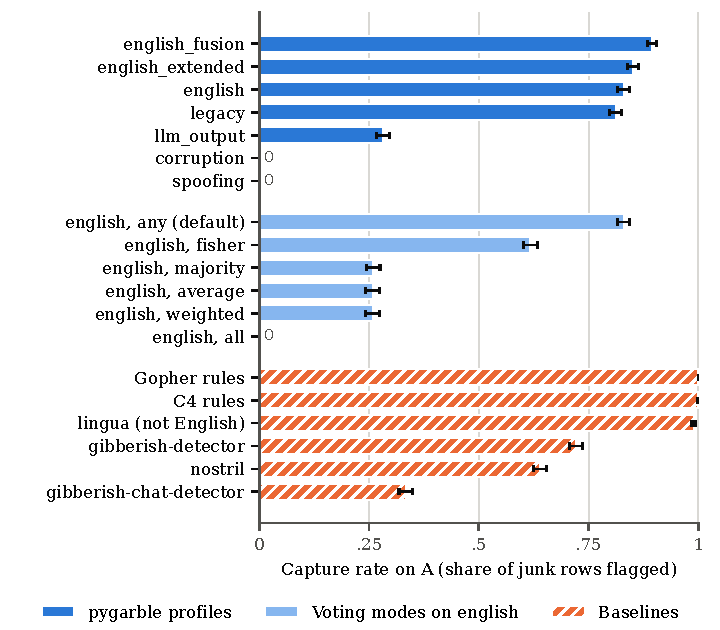
\includegraphics[width=0.8\linewidth]{figures/fig1_capture_a.pdf}
\caption{Capture rate on A (\nA{} survey responses labelled as junk), every
method at its default decision, with 95\,\% bootstrap intervals. Single
strategies are in Appendix~\ref{app:strategies}.}
\label{fig:capture}
\end{figure}

\begin{table}[t]
\centering
\small
\setlength{\tabcolsep}{4pt}
\caption{Capture rate on A and precision, recall and FPR on B at each
method's default decision, with 95\,\% bootstrap intervals. Precision is
n/a when a method flags nothing.}
\label{tab:results}
\resizebox{\linewidth}{!}{\begin{tabular}{lllll}
\toprule
Method & A capture & B precision & B recall & B FPR \\
\midrule
\multicolumn{5}{l}{\emph{pygarble profiles}} \\
english\_fusion & 0.895 {\scriptsize [0.884, 0.905]} & 0.906 {\scriptsize [0.898, 0.915]} & 0.991 {\scriptsize [0.987, 0.993]} & 0.068 {\scriptsize [0.062, 0.075]} \\
english & 0.830 {\scriptsize [0.817, 0.843]} & 0.656 {\scriptsize [0.645, 0.670]} & 0.947 {\scriptsize [0.940, 0.954]} & 0.332 {\scriptsize [0.320, 0.344]} \\
english\_extended & 0.852 {\scriptsize [0.839, 0.863]} & 0.649 {\scriptsize [0.638, 0.663]} & 0.951 {\scriptsize [0.944, 0.958]} & 0.344 {\scriptsize [0.331, 0.356]} \\
legacy & 0.812 {\scriptsize [0.798, 0.825]} & 0.781 {\scriptsize [0.770, 0.793]} & 0.947 {\scriptsize [0.940, 0.954]} & 0.178 {\scriptsize [0.169, 0.188]} \\
llm\_output & 0.282 {\scriptsize [0.267, 0.297]} & 0.200 {\scriptsize [0.184, 0.217]} & 0.110 {\scriptsize [0.100, 0.120]} & 0.294 {\scriptsize [0.282, 0.306]} \\
corruption & 0.000 {\scriptsize [0.000, 0.000]} & 0.000 {\scriptsize [0.000, 0.000]} & 0.000 {\scriptsize [0.000, 0.000]} & 0.285 {\scriptsize [0.274, 0.296]} \\
spoofing & 0.000 {\scriptsize [0.000, 0.000]} & n/a & 0.000 {\scriptsize [0.000, 0.000]} & 0.000 {\scriptsize [0.000, 0.000]} \\
\midrule
\multicolumn{5}{l}{\emph{Voting modes on english}} \\
english, any (default) & 0.830 {\scriptsize [0.817, 0.843]} & 0.656 {\scriptsize [0.645, 0.670]} & 0.947 {\scriptsize [0.940, 0.954]} & 0.332 {\scriptsize [0.320, 0.344]} \\
english, majority & 0.260 {\scriptsize [0.244, 0.275]} & 0.724 {\scriptsize [0.552, 0.880]} & 0.005 {\scriptsize [0.003, 0.008]} & 0.001 {\scriptsize [0.001, 0.002]} \\
english, all & 0.000 {\scriptsize [0.000, 0.000]} & n/a & 0.000 {\scriptsize [0.000, 0.000]} & 0.000 {\scriptsize [0.000, 0.000]} \\
english, average & 0.258 {\scriptsize [0.243, 0.274]} & 0.477 {\scriptsize [0.333, 0.630]} & 0.005 {\scriptsize [0.003, 0.008]} & 0.004 {\scriptsize [0.002, 0.005]} \\
english, weighted & 0.258 {\scriptsize [0.243, 0.274]} & 0.477 {\scriptsize [0.333, 0.630]} & 0.005 {\scriptsize [0.003, 0.008]} & 0.004 {\scriptsize [0.002, 0.005]} \\
english, fisher & 0.617 {\scriptsize [0.602, 0.634]} & 0.725 {\scriptsize [0.710, 0.741]} & 0.581 {\scriptsize [0.565, 0.595]} & 0.147 {\scriptsize [0.139, 0.156]} \\
\midrule
\multicolumn{5}{l}{\emph{Baselines}} \\
gibberish-detector & 0.722 {\scriptsize [0.707, 0.736]} & 0.995 {\scriptsize [0.993, 0.997]} & 0.822 {\scriptsize [0.809, 0.833]} & 0.003 {\scriptsize [0.002, 0.004]} \\
nostril & 0.640 {\scriptsize [0.624, 0.654]} & 0.975 {\scriptsize [0.968, 0.981]} & 0.550 {\scriptsize [0.534, 0.566]} & 0.010 {\scriptsize [0.007, 0.012]} \\
gibberish-chat-detector & 0.333 {\scriptsize [0.318, 0.349]} & 0.030 {\scriptsize [0.021, 0.040]} & 0.009 {\scriptsize [0.007, 0.013]} & 0.203 {\scriptsize [0.194, 0.214]} \\
lingua (not English) & 0.989 {\scriptsize [0.985, 0.992]} & 0.876 {\scriptsize [0.867, 0.886]} & 0.994 {\scriptsize [0.991, 0.996]} & 0.094 {\scriptsize [0.087, 0.101]} \\
Gopher rules & 1.000 {\scriptsize [1.000, 1.000]} & 0.401 {\scriptsize [0.392, 0.412]} & 1.000 {\scriptsize [1.000, 1.000]} & 1.000 {\scriptsize [1.000, 1.000]} \\
C4 rules & 0.999 {\scriptsize [0.999, 1.000]} & 0.402 {\scriptsize [0.392, 0.412]} & 1.000 {\scriptsize [1.000, 1.000]} & 0.998 {\scriptsize [0.997, 0.999]} \\
\bottomrule
\end{tabular}
}
\end{table}

\section{Results on social-media text}
\label{sec:social}

Figure~\ref{fig:pr} shows precision and recall on B. Recall is high for
most methods, because B's junk is random strings that share almost nothing
with English. \code{english\_fusion} recalls \res{english_fusion}{B_recall}
with precision \res{english_fusion}{B_precision}; it flags
\respct{english_fusion}{B_fpr}\,\% of tweets.

The precision differences come from tweets. gibberish-detector flags
\respct{gibberish_detector}{B_fpr}\,\% of tweets (precision
\res{gibberish_detector}{B_precision}) and nostril
\respct{nostril}{B_fpr}\,\%, both fewer than fusion; their recall is lower
(\res{gibberish_detector}{B_recall} and \res{nostril}{B_recall}). lingua
flags \respct{lingua}{B_fpr}\,\% of tweets. The \code{english} profile flags
\respct{english}{B_fpr}\,\%, \code{english\_extended}
\respct{english_extended}{B_fpr}\,\% and \code{legacy}
\respct{legacy}{B_fpr}\,\%. The Gopher and C4 rules flag
\respct{gopher_rules}{B_fpr}\,\% and \respct{c4_rules}{B_fpr}\,\% of tweets:
their word-count and line-structure rules were written for web documents,
and almost no tweet passes them.

\begin{figure}[t]
\centering
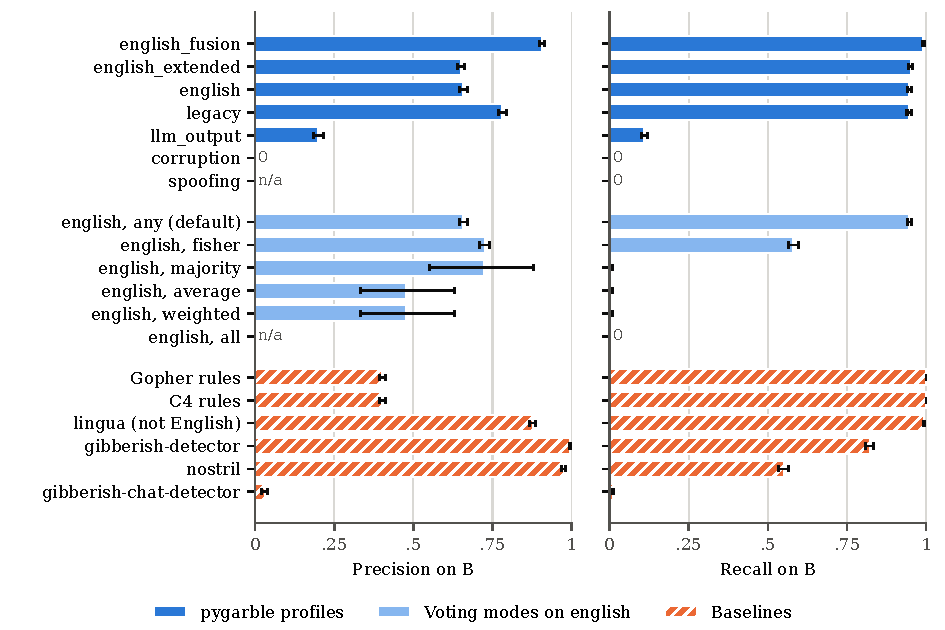
\includegraphics[width=\linewidth]{figures/fig2_precision_recall_b.pdf}
\caption{Precision and recall on B (\nBpos{} random strings, \nBneg{}
tweets), every method at its default decision, with 95\,\% bootstrap
intervals.}
\label{fig:pr}
\end{figure}

\section{Cost}

Figure~\ref{fig:cost} plots time against capture rate, and
Table~\ref{tab:footprint} lists time per 1,000 texts, import time and
install size, measured on one thread of an \cpuname{} with Python
\pyversion{} over all B texts (median of five runs after a warm-up).
\code{english\_fusion} takes \ms{english_fusion}\,ms per 1,000 texts and
pygarble installs in \mb{english_fusion}\,MB. gibberish-detector is faster
(\ms{gibberish_detector}\,ms) at \mb{gibberish_detector}\,MB, including the
corpus its model is trained from. lingua is the slowest (\ms{lingua}\,ms) and largest
(\mb{lingua}\,MB). All methods run offline once installed. Timings depend
on the machine; the ordering is what carries over.

\begin{figure}[t]
\centering
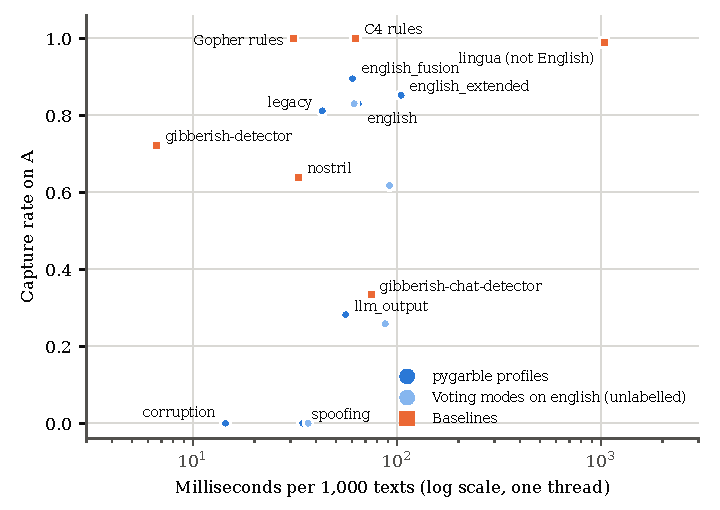
\includegraphics[width=0.8\linewidth]{figures/fig3_cost.pdf}
\caption{Milliseconds per 1,000 texts (log scale, one thread) against
capture rate on A. Voting modes are drawn but not labelled.}
\label{fig:cost}
\end{figure}

\begin{table}[t]
\centering
\small
\caption{Footprint. Time is the default decision over all \nB{} B texts on
one thread, median of five runs. Install size counts the installed files
of the distribution and its runtime dependencies, plus model or word-list
files the method needs.}
\label{tab:footprint}
\begin{tabular}{lrrr}
\toprule
Method & ms per 1,000 texts & Import (s) & Install (MB) \\
\midrule
\multicolumn{4}{l}{\emph{pygarble profiles}} \\
english\_fusion & 60.5 & 0.020 & 1.05 \\
english & 64.6 & 0.020 & 1.05 \\
english\_extended & 104.6 & 0.020 & 1.05 \\
legacy & 43.0 & 0.020 & 1.05 \\
llm\_output & 56.0 & 0.020 & 1.05 \\
corruption & 14.4 & 0.020 & 1.05 \\
spoofing & 34.4 & 0.020 & 1.05 \\
\midrule
\multicolumn{4}{l}{\emph{Voting modes on english}} \\
english, any (default) & 61.6 & 0.020 & 1.05 \\
english, majority & 87.4 & 0.020 & 1.05 \\
english, all & 36.7 & 0.020 & 1.05 \\
english, average & 86.0 & 0.020 & 1.05 \\
english, weighted & 87.5 & 0.020 & 1.05 \\
english, fisher & 91.7 & 0.020 & 1.05 \\
\midrule
\multicolumn{4}{l}{\emph{Baselines}} \\
gibberish-detector & 6.6 & 0.039 & 6.51 \\
nostril & 32.8 & 0.395 & 13.25 \\
gibberish-chat-detector & 74.6 & 0.036 & 20.63 \\
lingua (not English) & 1036.4 & 0.001 & 307.47 \\
Gopher rules & 30.9 & 0.003 & 0.01 \\
C4 rules & 62.5 & 0.003 & 0.01 \\
\bottomrule
\end{tabular}

\end{table}

\section{Where it fails}

This section lists every place where pygarble is beaten or weak.

\paragraph{False positives on informal text.} On tweets, the Markov
baseline gibberish-detector has an FPR of
\respct{gibberish_detector}{B_fpr}\,\% against \code{english\_fusion}'s
\respct{english_fusion}{B_fpr}\,\%, and nostril
\respct{nostril}{B_fpr}\,\%. Fusion catches more junk on both datasets, but at
default settings it is not the low-false-positive choice.

\paragraph{The default profile.} pygarble's default \code{english} profile
flags \respct{english}{B_fpr}\,\% of tweets, and \code{english\_extended}
\respct{english_extended}{B_fpr}\,\%. Under \code{any} voting a single
member firing is enough. Run alone, the control-character member flags
\respct{strategy_control_characters}{B_fpr}\,\% of tweets and the Markov
member \respct{strategy_markov_chain}{B_fpr}\,\%
(Appendix~\ref{app:strategies}); the first fires on the C1 control
characters inside mojibake (below). These profiles should not be used to
drop social-media text without calibration on the user's own data.

\paragraph{Language identification catches more survey junk.} lingua
captures \res{lingua}{A_capture} of A, more than any pygarble profile, by
calling anything it cannot identify as English junk. It pays with
\respct{lingua}{B_fpr}\,\% of tweets flagged, \mb{lingua}\,MB on disk and
the slowest time in Table~\ref{tab:footprint}, and it would flag every
non-English answer.

\paragraph{Short inputs and word-like mashes.} \code{english\_fusion}
misses \nAmissedfusion{} of the \nA{} rows in A. On inspection they are of
two kinds. Many are very short: single letters, digits, punctuation or a
few repeated letters, which give the English statistics too little
evidence. The rest are longer strings built from real words or
pronounceable fragments, which read as English to character and word
statistics. A minimum-length or character-class rule would catch the
first kind; nothing here catches the second reliably.

\paragraph{Profiles built for other junk.} \code{corruption} and
\code{spoofing} flag nothing in A, and \code{llm\_output} flags
\res{llm_output}{A_capture}. On B, \code{corruption} flags
\respct{corruption}{B_fpr}\,\% of tweets, because \mojibakepct\,\% of the
tweets contain mojibake byte signatures (for example a UTF-8 emoji decoded
as Windows-1252). Whether those flags are false positives depends on the
use: for an encoding audit they are correct, and B labels them clean only
because the dataset was built to separate random strings from tweets.
The same mojibake contributes to the FPR of the \code{english} profiles,
which include the mojibake check.

\paragraph{Conservative voting modes.} At the default threshold,
\code{majority}, \code{average} and \code{weighted} voting on the
\code{english} profile recall at most
\res{english_vote_majority}{B_recall} of B's random strings, and
\code{all} flags nothing. These modes need a lower threshold, chosen on
the user's data, before they are useful.

\paragraph{Label noise in A.} A is used as labelled. \nAmissedall{} rows
are flagged by none of the four English profiles, nostril,
gibberish-detector or lingua. On inspection many are meaningful but
low-effort answers, such as thanks or a short positive phrase, and the
rest are short mixes of words and fragments. A survey team may want to
discard the low-effort answers, but a gibberish detector should not flag
them, so A's capture rates have a ceiling below one.

\paragraph{B is easy for dictionary methods.} B's junk is random
character strings. A plain dictionary lookup separates them from tweets
almost perfectly: the \code{word\_lookup} strategy alone recalls
\res{strategy_word_lookup}{B_recall} of them with an FPR of
\respct{strategy_word_lookup}{B_fpr}\,\% (Appendix~\ref{app:strategies}).
B therefore says little about recall on realistic junk and mostly measures
false positives on informal English.

\section{Guidance}

\begin{itemize}
\item \textbf{Screening survey or form free text for review:}
  \code{english\_fusion}. It catches \res{english_fusion}{A_capture} of
  the junk answers in A at \ms{english_fusion}\,ms per 1,000 texts with no dependencies. Add a
  minimum-length rule for one- to five-character answers.
\item \textbf{Dropping rows automatically, where false positives cost more
  than misses:} at default settings, gibberish-detector's Markov model has
  the lowest FPR on tweets. Alternatively, calibrate an
  \code{english\_fusion} threshold with \code{calibrate()} on a few hundred
  labelled rows of your own data; this paper does not measure that option.
\item \textbf{Informal or social-media text:} avoid \code{english},
  \code{english\_extended} and \code{legacy} at default settings.
\item \textbf{Encoding damage:} \code{corruption}, knowing that it will
  flag mojibake that a human reader would call readable.
\item \textbf{Multilingual input:} none of the English profiles. Route by
  language first; a language identifier is the right tool for that
  question, not for junk detection.
\item \textbf{Short texts:} not the Gopher or C4 rules, which were designed
  for web documents and flag almost every tweet.
\end{itemize}

\section{Limitations}
\label{sec:limitations}

Two public datasets are measured, both English. A has only junk, so it
measures capture and nothing about false positives; B's junk is random
strings, which are easier than real junk. Both datasets are short texts;
pygarble's behaviour on long documents is not measured here. There is no
neural baseline. A comparison at a matched false-positive rate was
computed in PR~18 and removed from scope at the maintainer's direction; it
remains available in the repository history. Each method is run once at
its default decision, so the results say how the methods behave out of the
box, not how well they can be tuned.

\section{Reproducibility}

The benchmark code is in \code{paper/scripts/benchmark/}, the protocol and
every deviation from it in \code{paper/benchmark/}, and results in
\code{paper/benchmark/results/}. The manifest records the sha256 hash of
each raw file (for A, beginning \code{\shaA}) and every row id; no dataset
text is committed. Per-row scores and decisions for every method are
committed, so every number in this paper can be recomputed without the
raw data:
\begin{verbatim}
make benchmark-verify PYTHON=<venv>/bin/python
make preprint PYTHON=<venv>/bin/python
\end{verbatim}
The first command recomputes \code{metrics.json} from the saved predictions
and fails on any difference. The second regenerates the figures, the
tables and the number macros this paper is typeset from, then builds the
PDF. Re-scoring from the raw files is described in
\code{paper/scripts/benchmark/README.md}; scores are deterministic.

\section*{AI assistance}

Claude Code agents running Claude Opus 5.5, Claude Sonnet 5.5 and Claude
Fable 5.1 wrote the benchmark code, ran the experiments and drafted this
text, under the author's direction and review. Commit trailers in the
repository record the models used.

\bibliographystyle{plainnat}
\bibliography{references}

\appendix
\section{Single strategies}
\label{app:strategies}

Table~\ref{tab:strategies} shows each strategy run alone at its default
decision, sorted by capture rate on A. Intervals are in
\code{paper/benchmark/results/results.md}.

\begin{table}[h]
\centering
\small
\caption{Single strategies at their default decisions.}
\label{tab:strategies}
\begin{tabular}{lrrrrr}
\toprule
Strategy & A capture & B precision & B recall & B FPR & ms per 1,000 \\
\midrule
word\_lookup & 0.941 & 0.940 & 1.000 & 0.043 & 7.4 \\
markov\_chain & 0.801 & 0.781 & 0.947 & 0.178 & 30.9 \\
ngram\_frequency & 0.769 & 0.925 & 0.861 & 0.047 & 32.4 \\
pronounceability & 0.649 & 0.912 & 0.745 & 0.048 & 32.9 \\
log\_likelihood\_ratio & 0.624 & 0.999 & 0.725 & 0.000 & 36.4 \\
vowel\_ratio & 0.593 & 0.952 & 0.388 & 0.013 & 27.8 \\
word\_anomaly & 0.579 & 0.995 & 0.580 & 0.002 & 30.7 \\
pattern\_matching & 0.573 & 0.930 & 0.476 & 0.024 & 45.3 \\
cross\_parsing & 0.569 & 0.933 & 0.560 & 0.027 & 37.5 \\
ngram\_rank & 0.565 & 0.938 & 0.490 & 0.022 & 90.8 \\
keyboard\_pattern & 0.367 & 0.131 & 0.008 & 0.036 & 32.8 \\
consonant\_sequence & 0.365 & 0.984 & 0.190 & 0.002 & 7.9 \\
permutation\_test & 0.345 & 0.914 & 0.178 & 0.011 & 152.3 \\
keyboard\_adjacency & 0.320 & 0.388 & 0.006 & 0.007 & 12.9 \\
primed\_compression & 0.270 & 0.970 & 0.404 & 0.008 & 65.5 \\
entropy\_based & 0.259 & 0.986 & 0.054 & 0.001 & 24.2 \\
local\_anomaly & 0.207 & 0.989 & 0.110 & 0.001 & 31.6 \\
letter\_position & 0.191 & 0.544 & 0.022 & 0.012 & 29.1 \\
letter\_frequency & 0.179 & 0.000 & 0.000 & 0.010 & 29.6 \\
repetition & 0.119 & 0.000 & 0.000 & 0.015 & 17.1 \\
bigram\_probability & 0.092 & 1.000 & 0.153 & 0.000 & 13.5 \\
rare\_trigram & 0.020 & 1.000 & 0.019 & 0.000 & 9.5 \\
function\_word\_density & 0.019 & 0.000 & 0.000 & 0.029 & 6.1 \\
vowel\_pattern & 0.012 & 0.105 & 0.001 & 0.006 & 7.1 \\
word\_collocation & 0.008 & 0.000 & 0.000 & 0.039 & 8.2 \\
hex\_string & 0.008 & 0.000 & 0.000 & 0.008 & 6.8 \\
symbol\_ratio & 0.002 & 0.000 & 0.000 & 0.002 & 4.6 \\
affix\_detection & 0.002 & n/a & 0.000 & 0.000 & 22.5 \\
control\_characters & 0.000 & 0.000 & 0.000 & 0.284 & 8.3 \\
mojibake & 0.000 & 0.000 & 0.000 & 0.094 & 7.3 \\
unicode\_script & 0.000 & n/a & 0.000 & 0.000 & 34.2 \\
zipf\_conformity & 0.000 & n/a & 0.000 & 0.000 & 3.2 \\
\bottomrule
\end{tabular}

\end{table}

\end{document}
